\documentclass{report}
%Math Stuff
\usepackage{amsmath}
\usepackage{enumitem}
\usepackage{mathtools}

%General Formating
\usepackage[letterpaper, portrait, margin=1in]{geometry}
\usepackage{fancyhdr}
\pagestyle{fancy}

%Bibliography
\usepackage[toc,page]{appendix}

%Figures
\usepackage{graphicx}
\graphicspath{ {figures/} }
\usepackage{tikz}
\usepackage{pgfmath}
\usepackage{framed}
\usepackage{csvsimple}

%Header
\lhead{Schulman}
\rhead{Page \thepage}

%Title
\title{Food Networks \\~\\ \normalsize A Thesis Presented to the Faculty of the Economics Department of Cornell University in Partial Fulfillment of the Requirements for the Degree of Bachelor of Arts in Economics with Honors} 
\author{Eric Schulman}
\date{May 2017}

\begin{document}

\maketitle

\tableofcontents

\pagebreak

\begin{abstract}
For my thesis, I ask how produce prices relate to the structure of the network of farms, intermediate buyers, and stores. To answer this question, I estimate the relative cost of transporting grapes, cabbage, onions, and cherries in to each census tract in New York State. My estimates come from an optimization problem specified using publicly available sattelite data regarding crop cover and New York's records on food vendor permits. I solve the problem using linear programming software packages. All of the code to used to complete this project is publicly available on GitHub.

\end{abstract}

\chapter{Background}

\section{Related Work}

\subsection{Demographics, Policy and Nutrition}

Researchers have studied the statistical relationship between transfer programs, demographics and nutritional outcomes for a long time. Calculating these statistical relationships is straightforward for the US because the Census Bureau publishes a monthly current population survey monthly and nutrition supplement. 

This literature finds reducing costs and increasing availability of nutritional foods improves health outcomes. One study evaluated the Farmers' Market Nutrition Program, a national program intended to increase consumption of fresh fruits and vegetables by providing coupons and information. Researchers found subsidizing nutritionally rich food with coupons leads to increased consumption when complemented with information \cite{Just}. The literature also found nutritional outcomes are related to systemic factors. For example, researchers analyzed nutritional outcomes in Oregon between 1999 and 2001, when Oregon had the highest average rate of hunger in the nation. The study found county-level factors like residential location and housing costs were most related to food insecurity \cite{Bernell}. 


\subsection{Spatial Data and Nutrition}

Researchers realized state-level data has its limitations limitations. To understand systemic nutritional patterns, researchers began describing food supply in detail using spatial coordinates and mapping software.  One study conducted among grocery stores across inner cities and suburbs within the Minneapolis and St. Paul metropolitan concluded the urban poor pay marginally more for food because supermarket chains don't open in inner cities \cite{Chung}. Researchers began applying the label "food deserts" to inner cities. With more data becoming available online, researchers continue describing food supply in more detail to understand systemic food insecurity. In one project, researchers leveraged Google Maps, and local online news to build a graphical representation of food availability in Bogota, Columbia \cite{Hwang}. Another study used online directories of grocery stores to index neighborhoods' vulnerability to food insecurity in the twin cities area \cite{Larson}.
 
\subsection{Optimization Problem and Food}

Food allocation is closely related with nutrition and often studied using a transportation problem. Transportation problems are an optimization problem designed to find the cheapest possible way of sending a certain amount of supply through a network. A typical application of this problem involves finding the best delivery route from a factory to a warehouse where the road network has some capacity and cost associated. Solving the problem involves finding a vector with an economic interpretation of optimal prices from a social planning perspective. It can be solved efficiently using the network simplex algorithm and linear programming software packages \cite{Cook}. Researchers have often applied transportation problems to food allocation. One paper studies maize allocation in South Africa where rails carry maize from supply and demand points, scattered throughout the country. Researchers minimize the total rail cost, as is standard, but add a secondary objective of distributing costs fairly among all users \cite{Stewart}.

\section{Optimal Transportation}

I've decided to devote a section of my thesis explaining the nature of the optimization problem I specify and solve. My chosen application for the transportation problem is novel, but the problem its self is not. It's actually taught in most undergraduate optimization courses. Since I recognize that this is a different direction than projects from the past, I want to make sure it's clear what I've done and the tools that I used to do it.

\subsection{Problem Description}

The optimization problem plan to specify and solve is called a transportation problem. It actually has a few names. It's usually called minimum-cost flow. This is because the it tries to maximize the amount of flow (in my case units of goods flowing through a network) at the minimum cost. I've decided to refer to it as a transportation problem because of how I'm using it. It's essentially a more general version of a matching market. There are suppliers and demand-ers connected in a network. Like a matching market, the goal is to match supply with demand. The catch is that edges in this problem are not all equal. Certain edges are more expensive than others. The difference betweeen this and a normal matching market is that this problem tries to find the cheapest possible way to match supply with demand. The problem inputs are list of suppliers and demand-ers with capacities and edges with costs. It tells you how much of each good each supplier should send to each demand-er.

\subsection{Solving the Problem}

Finding the minimum cost of sending goods through the network works a lot like finding the optimal matching for a matching market. You can start by maximizing the amount of goods you've sent through the network without worrying about cost. This works exactly like a normal matching market. You can use the augmenting path to do this. After finding the maximum amount of goods flowing through the network, the algorithm tries to find the optimal cost. You do so by finding a reduced cost path. This works exactly like an augmenting path in a matching market. You start at a supply node and trace a path alternating between supply and demand until you reach your original node. If you can trace back to your initial node then you've reduced the cost. You repeat this process until you've exhausted all of the reduced cost cycles.


\subsection{Worked out Example}

To get a better sense of the problem and how to solve it, I've worked out an example of a transportation problem with a network of 5 nodes.

\begin{figure}
\centering
\begin{framed}
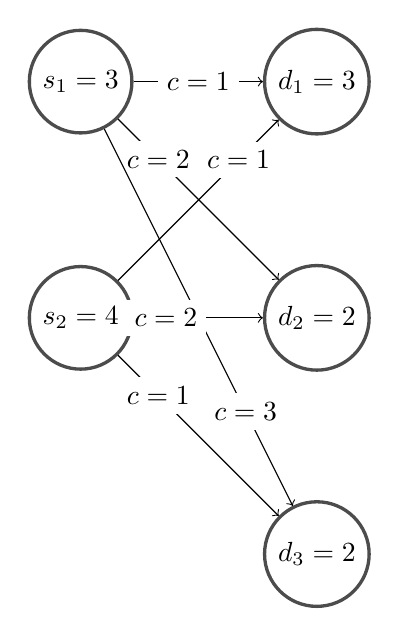
\begin{tikzpicture}[
node/.style={circle, draw=black!70, fill=white!5, very thick, minimum size=9mm}
]
%Nodes
\node[node]      (s1)                                        {$s_1= 3$};
\node[node]      (s2)     [below of =s1, yshift= -2cm]       {$s_2 = 4$};
\node[node]      (d1)     [right of =s1 , xshift= 2cm]       {$d_1 = 3$};
\node[node]      (d2)     [below of = d1, yshift= -2cm]       {$d_2 = 2$};
\node[node]      (d3)     [below of = d2, yshift= -2cm]      {$d_3 = 2$};
%Lines
\draw[->] (s1) -- (d1) node [midway, fill=white] {$c= 1$};
\draw[->] (s1) -- (d2) node [near start, fill=white] {$c = 2$};
\draw[->] (s1) -- (d3) node [near end, fill=white] {$c = 3$};
\draw[->] (s2) -- (d1) node [near end, fill=white] {$c = 1$};
\draw[->] (s2) -- (d2) node [near start, fill=white] {$c = 2$};
\draw[->] (s2) -- (d3) node [near start, fill=white] {$c = 1$};
\end{tikzpicture}
\caption{This picture represents the network for which we will be finding minimum cost flow. The supply and demand nodes are labeled with their corresponding capacities.  The edges between each supply and demand node are labled according to their cost. To make the problem easier, you can assume all edges have unlimited capacity meaning suppliers can send as much goods as they want over them.}
\end{framed}
\end{figure}

\begin{figure}
\centering
\begin{framed}
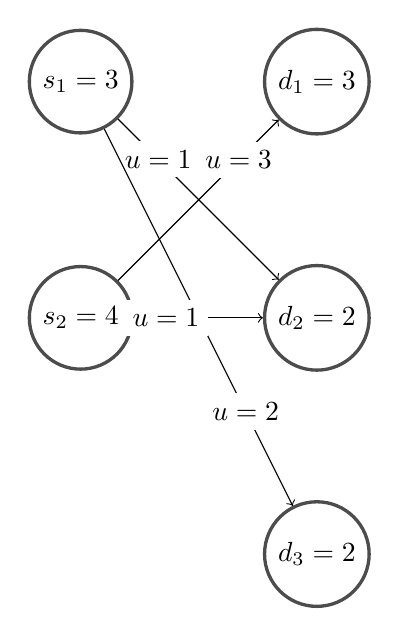
\begin{tikzpicture}[
node/.style={circle, draw=black!70, fill=white!5, very thick, minimum size=9mm}
]
%Nodes
\node[node]      (s1)                                        {$s_1= 3$};
\node[node]      (s2)     [below of =s1, yshift= -2cm]       {$s_2 = 4$};
\node[node]      (d1)     [right of =s1 , xshift= 2cm]       {$d_1 = 3$};
\node[node]      (d2)     [below of = d1, yshift= -2cm]       {$d_2 = 2$};
\node[node]      (d3)     [below of = d2, yshift= -2cm]      {$d_3 = 2$};
%Lines
\draw[->] (s1) -- (d2) node [near start, fill=white] {$u = 1$};
\draw[->] (s1) -- (d3) node [near end, fill=white] {$u = 2$};
\draw[->] (s2) -- (d1) node [near end, fill=white] {$u = 3$};
\draw[->] (s2) -- (d2) node [near start, fill=white] {$u = 1$};
\end{tikzpicture}
\caption{The algorithm starts by matching the capacities on the supply nodes with the capacities on the demand nodes. This is trivial because there are no edge capacities and every node is connected.}
\end{framed}
\end{figure}

\begin{figure}
\centering
\begin{framed}
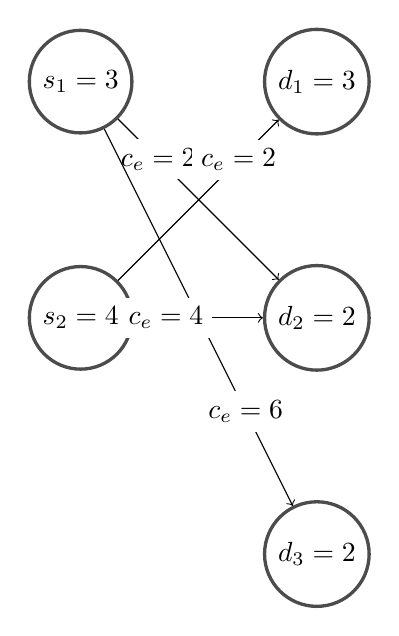
\begin{tikzpicture}[
node/.style={circle, draw=black!70, fill=white!5, very thick, minimum size=9mm}
]
%Nodes
\node[node]      (s1)                                        {$s_1= 3$};
\node[node]      (s2)     [below of =s1, yshift= -2cm]       {$s_2 = 4$};
\node[node]      (d1)     [right of =s1 , xshift= 2cm]       {$d_1 = 3$};
\node[node]      (d2)     [below of = d1, yshift= -2cm]       {$d_2 = 2$};
\node[node]      (d3)     [below of = d2, yshift= -2cm]      {$d_3 = 2$};
%Lines
\draw[->] (s1) -- (d2) node [near start, fill=white] {$c_e = 2$};
\draw[->] (s1) -- (d3) node [near end, fill=white] {$c_e = 6$};
\draw[->] (s2) -- (d1) node [near end, fill=white] {$c_e = 2$};
\draw[->] (s2) -- (d2) node [near start, fill=white] {$c_e = 4$};
\end{tikzpicture}
\caption{This solution is not optimal in terms of cost (yet). I've labled each edge in this figure with the cost each edge has incurred. It works out to 14. The edge costs are just the amount of flow on each edge times its cost.}
\end{framed}
\end{figure}

\begin{figure}
\centering
\begin{framed}
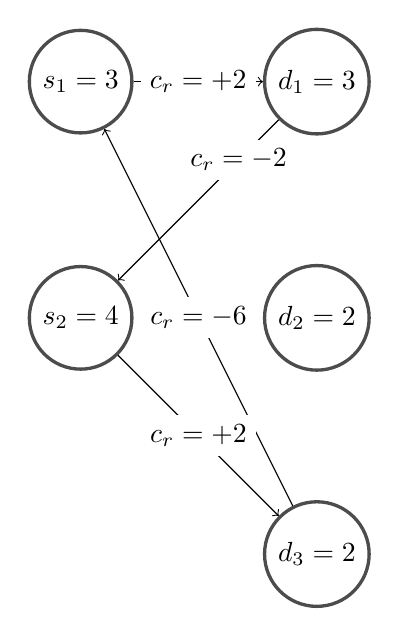
\begin{tikzpicture}[
node/.style={circle, draw=black!70, fill=white!5, very thick, minimum size=9mm}
]
%Nodes
\node[node]      (s1)                                        {$s_1= 3$};
\node[node]      (s2)     [below of =s1, yshift= -2cm]       {$s_2 = 4$};
\node[node]      (d1)     [right of =s1 , xshift= 2cm]       {$d_1 = 3$};
\node[node]      (d2)     [below of = d1, yshift= -2cm]       {$d_2 = 2$};
\node[node]      (d3)     [below of = d2, yshift= -2cm]      {$d_3 = 2$};
%Lines
\draw[->] (s1) -- (d1) node [midway, fill=white] {$c_r=+2$};
\draw[<-] (s1) -- (d3) node [midway, fill=white] {$c_r= -6$};
\draw[<-] (s2) -- (d1) node [near end, fill=white] {$c_r=-2 $};
\draw[->] (s2) -- (d3) node [midway, fill=white] {$c_r=+2$};
\end{tikzpicture}
\caption{In order to improve the cost of flow through the network, we look for a reduced cost cycle. The cycle needs to start and end on the same node. It also needs to alternate between suppliers and demand nodes. This is because you delete costly edges and replace them with less expensive ones. By traversing the cycle we see can reduce the cost by 4 to the optimal amount. Edges in the cycle are labled with their reduced cost (i.e. how much they improve the total cost)}
\end{framed}
\end{figure}

\begin{figure}
\centering
\begin{framed}
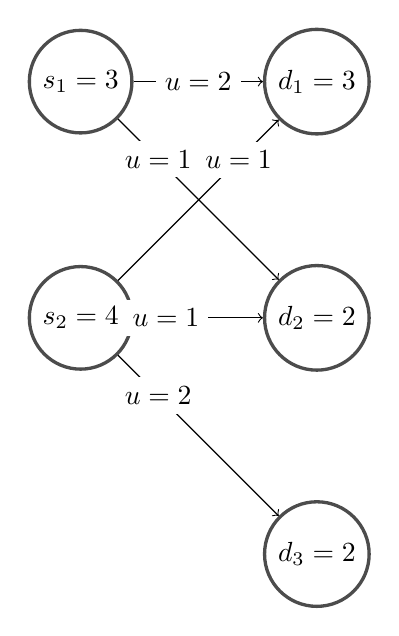
\begin{tikzpicture}[
node/.style={circle, draw=black!70, fill=white!5, very thick, minimum size=9mm}
]
%Nodes
\node[node]      (s1)                                        {$s_1= 3$};
\node[node]      (s2)     [below of =s1, yshift= -2cm]       {$s_2 = 4$};
\node[node]      (d1)     [right of =s1 , xshift= 2cm]       {$d_1 = 3$};
\node[node]      (d2)     [below of = d1, yshift= -2cm]       {$d_2 = 2$};
\node[node]      (d3)     [below of = d2, yshift= -2cm]      {$d_3 = 2$};
%Lines
\draw[->] (s1) -- (d1) node [midway, fill=white] {$u=2$};
\draw[->] (s1) -- (d2) node [near start, fill=white] {$u=1$};
\draw[->] (s2) -- (d1) node [near end, fill=white] {$u=1$};
\draw[->] (s2) -- (d2) node [near start, fill=white] {$u=1$};
\draw[->] (s2) -- (d3) node [near start, fill=white] {$u=2$};
\end{tikzpicture}
\caption{At this point, there are no more reduced cost cylces, so we've found an optimal solution in terms of cost. The edges reflect the amount of units flowing from supply to demand in this solution.}
\end{framed}
\end{figure}

\begin{figure}
\centering
\begin{framed}
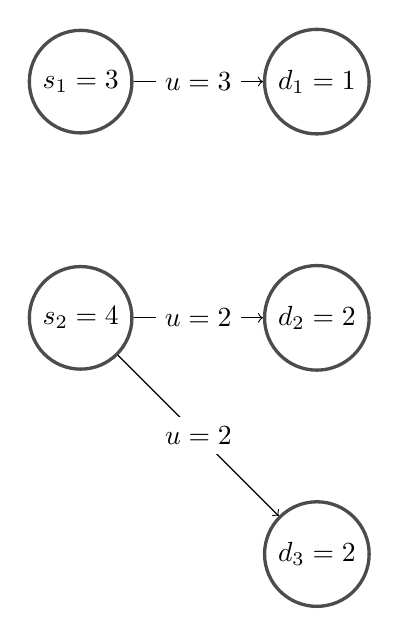
\begin{tikzpicture}[
node/.style={circle, draw=black!70, fill=white!5, very thick, minimum size=9mm}
]
%Nodes
\node[node]      (s1)                                        {$s_1= 3$};
\node[node]      (s2)     [below of =s1, yshift= -2cm]       {$s_2 = 4$};
\node[node]      (d1)     [right of =s1 , xshift= 2cm]       {$d_1 = 1$};
\node[node]      (d2)     [below of = d1, yshift= -2cm]       {$d_2 = 2$};
\node[node]      (d3)     [below of = d2, yshift= -2cm]      {$d_3 = 2$};
%Lines
\draw[->] (s1) -- (d1) node [midway, fill=white] {$u=3$};
\draw[->] (s2) -- (d2) node [midway, fill=white] {$u=2$};
\draw[->] (s2) -- (d3) node [midway, fill=white] {$u=2$};
\end{tikzpicture}
\caption{As long as there aren't minimum cost cylces we've found a solution. Zero-cost cycles exists in this simple network. As a result, there is more than 1 solution that optimizes cost and flow. This figure shows that example.}
\end{framed}
\end{figure}

\section{Linear Programming}

\subsection{The Simplex Algorithm}

There are a few ways to solve this problem. Because I have a lot of variables I want to solve for, I plan on specifying this problem as linear program and solving it with the simplex algorithm. This algorithm is essentially like the ordinary least squares of optimization. People have written textbooks describing it's properties and variation. A quick google search would do a better job of explaining than me, but I'll try any way. The algorithm finds the solution to a linear objective (i.e. $a x_1 +b x_2 + ...$ ) subjected to linear constraints. The intuition behind how it works is that it states the problem in two ways and finds the lowest maximum and highest minimum. When these happen to coincide,  you know you've found a maximum. At first glance, the  linear nature of the problem function might look like OLS, but they are very different. In OLS, the estimated coefficinets are used to approximate some variable of interests. In linear programming, you get point values for each of the variables of interest to minimize the objective function.

\section{Primal Problem}

In order to use linear programming packages, we need to formally state the problem. The statement is fairly intuitive. As we said before, the problem tries to send as much units of a good from a suppliers $s$ in the set $S$ to demanders $d$ in the set $D$. However, there are costs for sending a unit of good across every route between suppliers and demand-ers. We want to minimize these costs which leads to our objective function (in the objective $c$ is costs and $u$ is units of the good).

$$\operatorname{Minimize} \sum_{s,d \in \text{Routes}} c_{s,d} u_{s,d}$$

The constraints on the objective function reflect the fact that supply and demand must should balance. The first set of contraints require that demand be satisfied.

$$\sum_{s,d \in \text{Routes}} \text{u}_{s,d}= \text{demand at } d \text{ (for all demand-ers } s \in S)$$

The second set of constraint requires that no supply goes to waste. In other words, no product is just left at suppliers. In this case, supply is a negative quantity because supply leaves the supply nodes and flows to demand nodes.

$$\sum_{s,d \in \text{Routes}} \text{u}_{s,d}= \text{supply at } s \text{ (for all suppliers } d \in D)$$

Finally, we can't have negative amounts of units flow across the routes.

$$0 \leq u_{s,d}, \forall s,d \in \text{Routes}$$

Putting it all together, supply in demand balance because suppliers are required to send a certain amount of flow and demand-ers must receive a certain amount.
$$\operatorname{Minimize} \sum_{s,d \in \text{Routes}} c_{s,d} u_{s,d}$$
$$\text{subject to}$$
$$\sum_{s,d \in \text{Routes}} \text{u}_{s,d}= \text{demand at } d \text{ (for all suppliers } s \in S)$$
$$\sum_{s,d \in \text{Routes}} \text{u}_{s,d}= \text{supply at } s \text{ (for all demand-ers } d \in D)$$
$$0 \leq u_{s,d}, \forall s,d \in \text{Routes}$$

To summarize, the objective function minimizes total costs. The first and second constraints ensure nodes either produce or consume based on their type; the third ensures supply moves forward from supply to demand.  In the case, when supply doesn't equal demand you can add an extra node to the problem. You let other nodes send supply or recieve goods from this node at 0 cost (depending on whether there is too much supply or demand). The amount flow from this node to others represents a shortage or surplus.


\section{Dual Problem}

Every linear program has an equivalent dual problem. In the dual, the constraints become the variables of interest and the variables of interest become constraints. The intuition behind the dual problem for the transportation problem comes from the desire to get rid of augmenting cycles. The dual formalizes this idea.

Essentially we introduce a slack variable at each node $p$. When we compute the costs of cycles we can trivially add and subtract $p$ at each node. As long as the slack variables cancel we haven't changed the nature of the problem. However, since this is a slack variable, it can take what ever value we want. We can use it to encode the amount by which firms "missed the mark" from the optimal solution. For this reason, in the optimal solution we want

$$ p_d -p_s - c_{s,d}\leq 0$$

If this holds then we know we know that we've found the optimal solution. It helps to think of the dual variable and a price. Firms $s$ earns $p_d$ for sending their product to $d$ but looses $p_s + c_{s,w}$. The constraint prevents arbitrage through the network. If it didn't hold, all the firms would send their product across this edge.

$$\operatorname{Maximize} \sum_{d \in D}  (\text{demand at } d) \cdot p_{d} -   \sum_{s \in S}  (\text{supply at } s) \cdot p_{s} $$

$$ -p_s + p_d \leq c_{s,d}, \forall s,d\in \textrm{Routes}$$

Putting it together we have

$$\operatorname{Maximize} \sum_{d \in D}  (\text{demand at } d) \cdot p_{d} -   \sum_{s \in S}  (\text{supply at } s) \cdot p_{s} $$
$$ \text{ subject to}$$
$$ -p_s + p_d \leq c_{s,d}, \forall s,d\in \textrm{Routes}$$

The dual problem actually yields a more interesting economic description of the system. Basically, instead of finding the amount of units sent between each pair of suppliers and demand-ers, we can look prices that reflect the relative cost of sending goods to certain demanders.

The dual variable $p_v$ can be interpreted as optimal prices from a social planning perspective. The problem maximizes profits from a social planning perspective. The constraint that arbitrage profits do not exist in the network. The price you pay at the demand node $p_d$, cannot exceed the price you pay at the supplier $p_s$ plus the cost of sending the unit of good $c_{d,s}$. This has to do with the fact that the algorithm completes when the reduced costs cycles are exhausted.

\subsection{Characterizing Solutions}

As an economist, I would hope you are skeptical of any solution to this problem involving supply and demand found by the simplex algorithm. First of all, I am making point estimates as opposed to 

The algorithm can actually return more than one solution. Going back to the previous example, You can see that the problem actually has more than one Solution.

\subsection{Software}
In order to actually solve the problem, I had to write a bit of code. Specifically, solving the optimization problem involved installing a software package that implemented the simplex algorithm. Additionally, since the results produce point estimates, a matrix with 5000 prices isn't readable. As a result, I wrote code to parse some descriptive statistics from the solution files.

I'm a big believer in open source code. As a result, I've made all the code I wrote for this project publicly available on GitHub with a detailed explanation about how to get it running. Since open source is important to me, most of the software dependencies that need to be installed in order to get my code working are open source. The one exception is the linear optimizer. In this case, I used Gurobi which is free with an academic license.

\subsection{Computational Complexity}
A final thing worth mentioning is the efficiency of the simplex algorithm (i.e. comp. However, measuring a programs efficiency by factors like how long it takes to run or how many lines of code it takes can vary with the computer and the compiler. It is also variable with the input to the program. As a result, in order to have a more universal measure of efficiency Computer scientists measure efficiency using run-time bounds. Basically, run-time bounds tell you an upper bound on the number of steps you need to solve the problem, given the input.

The simplex algorithm's run time bound is actually very bad as far as we know. It can be $O(2^n)$. Meaning that if there $2^n$ inputs, the number of instructions is some factor of $2^n$. Proving that it has a low average run time bound is an area of active research. The general rule of thumb is that the simplex algorithm has a run time that is some polynomial of $n$.

\chapter{Problem Specification}

For each crop, New York has farms, agricultural dealers and food retailers. In the problem, farms send their goods to intermediaries and which in turn send their crop to stores purely based on transportation cost. Exports are assumed to be insignificant. Farms, intermediaries, and vendors incur transportation costs equals to the expected travel time between them. Farms can ship to any intermediary associated with the same crop and intermediaries can ship to any store. Intermediaries can scale as much as they desire. Farms produce agricultural products proportional to their size. Stores satisfy demand proportional to the market value of their square footage. 

The I chose to look at the classification XX

I chose to group by census tracts, these are roughly muncipal level.

You can see the amount of sq footage alotted to each tract

here you can see the stores, the color indicates their relative size. I've put the census tracts behind them

below is the census tracts with the median household income.

\begin{figure}
\centering
\begin{framed}
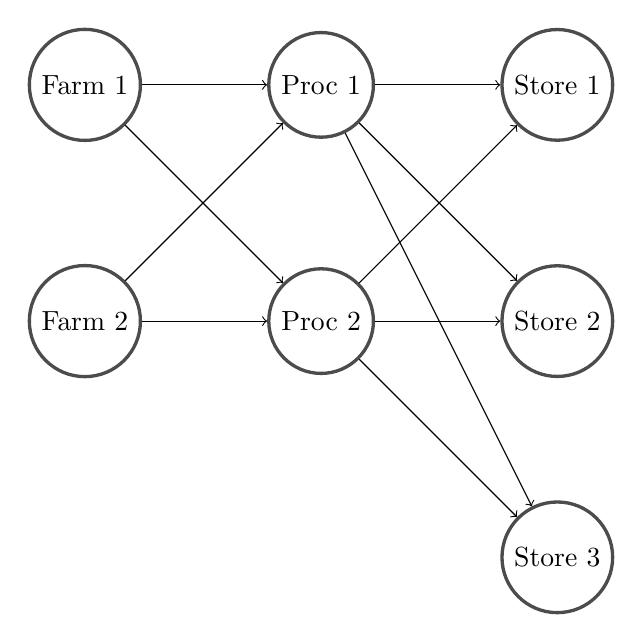
\begin{tikzpicture}[
node/.style={circle, draw=black!70, fill=white!5, very thick, minimum size=9mm}
]

%Nodes
\node[node]      (f1)                                        {Farm 1};
\node[node]      (f2)     [below of = f1, yshift= -2cm]       {Farm 2};
\node[node]      (p1)    [right of = f1, xshift= 2cm]        {Proc 1};
\node[node]      (p2)     [below of =p1, yshift= -2cm]       {Proc 2};
\node[node]      (s1)     [right of = p1 , xshift= 2cm]       {Store 1};
\node[node]      (s2)     [below of = s1, yshift= -2cm]       {Store 2};
\node[node]      (s3)     [below of = s2, yshift= -2cm]      {Store 3};
 
%Lines
\draw[->] (f1) -- (p1) ;%node [midway, fill=white] {};
\draw[->] (f1) -- (p2) ;%node [near start, fill=white] {};
\draw[->] (f2) -- (p1) ;%node [near start, fill=white] {distance};
\draw[->] (f2) -- (p2) ;%node [midway, fill=white] {distance};
\draw[->] (p1) -- (s1) ;%node [midway, fill=white] {distance};
\draw[->] (p1) -- (s2) ;%node [near start, fill=white] {distance};
\draw[->] (p1) -- (s3) ;%node [near end, fill=white] {distance};
\draw[->] (p2) -- (s1) ;%node [near end, fill=white] {distance};
\draw[->] (p2) -- (s2) ;%node [midway, fill=white] {distance};
\draw[->] (p2) -- (s3) ;%node [near start, fill=white] {distance};
\end{tikzpicture}
\caption{This shows something}
\end{framed}
\end{figure}


\section{Reduction to Minimum Cost Flow}

A common thing to do in computer science is to change one complicated problem you may not know how to solve into a simpler one you can solve. When you prove the two problems are equivalent you have "reduced" the more complex problem to the simpler one. In my case, I want to show that the problem I've specified above can be specified as a linear program which I can solve with the simplex algorithm.

A transportation problem is a natural framework for New York's agricultural supply network. Supply nodes are farms and demand nodes are stores.  The transportation problem assumes that supply and demand balance. Since New York exports agricultural products, I add a special demand node with demand equal to New York's net exports for each crop. Farms send goods to this node at no cost. This is equivalent to my original problem which also ignored exports. 

$$\operatorname{Minimize} \sum_{f,p \in \text{Routes}} c_{f,p} u_{f,p} + \sum_{p,s \in \text{Routes}} c_{p,s} u_{p,s}$$
$$\text{subject to}$$
$$\sum_{f,p \in \text{Routes}} \text{u}_{f,p}= \text{supply at } f \text{ (for all farms } f \in F)$$
$$\sum_{f,p \in \text{Routes}} \text{u}_{f,p} + \sum_{p,s \in \text{Routes}} \text{u}_{p,s} = 0 \text{ (for all processors } p \in P)$$
$$\sum_{p,s \in \text{Routes}} \text{u}_{p,s}= \text{demand at } s \text{ (for all stores } s \in S)$$
$$0 \leq u_{s,d}, \forall s,d \in \text{Routes}$$


All we need to do is 

\section{Dual Problem Formulation}

Of course, I will be solving the dual problem, not the primal to find prices. The dual problem I've formulated is

$$\operatorname{Maximize} \sum_{s \in S}  (\text{demand at } s) \cdot p_{s} -   \sum_{f \in F}  (\text{supply at } f) \cdot p_{f} $$
$$ \text{ subject to}$$

We need two sets of constraints, one for the edges between the farms and processorsm, and another for the edges between the processors and stores. They are stated below.

$$ -p_f + p_p \leq c_{f,p}, \forall f,p\in \textrm{Routes}$$
$$ -p_p + p_s \leq c_{p,s}, \forall p,s\in \textrm{Routes}$$

\section{Data Sources}

\subsection{Farms}

My data on acreage and location comes from a GeoTIFF image created by satellite pictures from the National Agricultural Statistical Service. The file forms a grid. Each square represents a 900 square meter plot labeled according the crop growing. I will convert continuous stretches of pixels into polygons representing farms and assign locations to farms based on each polygon's centroid. I normalize the size of farms based on their size in pixels as a share of each crops' output. For some crops, the pixel accuracy can be as low as 50 percent. I am looking into ways to improve this.
Landsat represents the world's longest continuously acquired collection of space-based moderate-resolution land remote sensing data. Four decades of imagery provides a unique resource for those who work in agriculture, geology, forestry, regional planning, education, mapping, and global change research. Landsat images are also invaluable for emergency response and disaster relief.
The USDA, NASS Cropland Data Layer (CDL) is a raster, geo-referenced, crop-specific land cover data layer. The 2010 CDL has a ground resolution of 30 meters. The CDL is produced using satellite imagery from the Landsat 5 TM sensor, Landsat 7 ETM+ sensor, and the Indian Remote Sensing RESOURCESAT-1 (IRS-P6) Advanced Wide Field Sensor (AWiFS) collected during the current growing season. Some CDL states used additional satellite imagery and ancillary inputs to supplement and improve the classification.

\begin{table}
\centering
\begin{framed}
\begin{tabular}{c|c|c|c|c}%
	Type&Band&Correct Pixels&Accuracy&Omission Error
    \csvreader[head to column names]{band.csv}{}% use head of csv as column names
    {\\\hline \csvcoli & \csvcolii & \csvcoliii & \csvcoliv& \csvcolv}
\end{tabular}
\caption{Another table caption}
\end{framed}
\end{table}

The Cropland Data Layer (CDL) is produced using agricultural training data from the Farm Service Agency (FSA) Common Land Unit (CLU) Program and non-agricultural training data from the United States Geological Survey (USGS) National Land Cover Dataset 2001 (NLCD 2001)





\subsection{Intermediate Processors}
The connection between produce and nutrition isn't the only reason I focus my analysis on produce. Produce isn't drastically altered during intermediate processing. According to New York States' records on agricultural supplier permits there are roughly 300 licensed agricultural product dealers. New York State requires farm product vendors who buy more than 10,000 dollars in farm products to register for a license annually. By registering they disclose what crops they sell and their location. I use this information to include intermediate nodes in the transportation problem for their corresponding crop.
There are actually a few from out of state, I've dropped these observations


\subsection{Stores}

New York State keeps a ledger detailing the locations and sizes of of farmers markets and stores. There are roughly 700 farmers markets held in the state. This data includes GPS coordinates. The food retail establishment data includes 30,000 registered food vendors. For my analysis, I exclude certain classifications of stores like bakers and meat markets. The data includes labels for filtering purposes. I use stores' addresses to determine their GPS coordinates using MapQuest. In my model, stores' share of total consumption equals the cost of their square footage as share of the total. The data on property values comes from the Census's 2010 American Community Survey.

The store data set has roughly 20,000 different stores with the classification involved with selling produce.

This map show, all of the stores mapped. They've been overlayed to the census tract so you can get a sense of how many of them there are

\begin{figure}
\centering
\begin{framed}
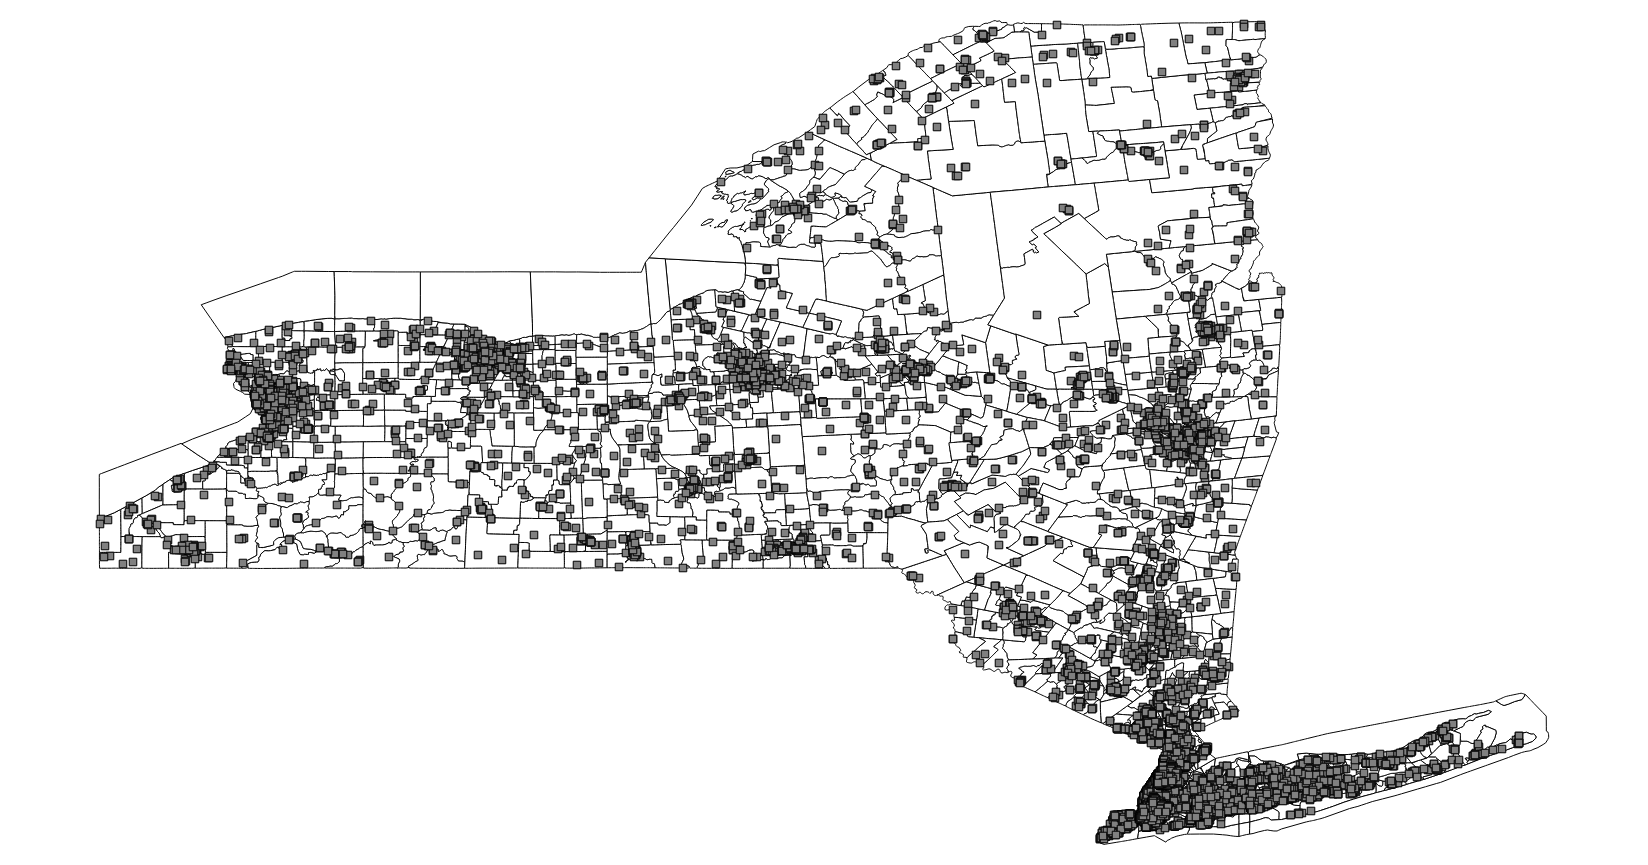
\includegraphics[scale=.4]{map_3}
\caption{This shows something}
\end{framed}
\end{figure}

This map shows the distribution of incomes through out the census tracts.

\begin{figure}
\centering
\begin{framed}
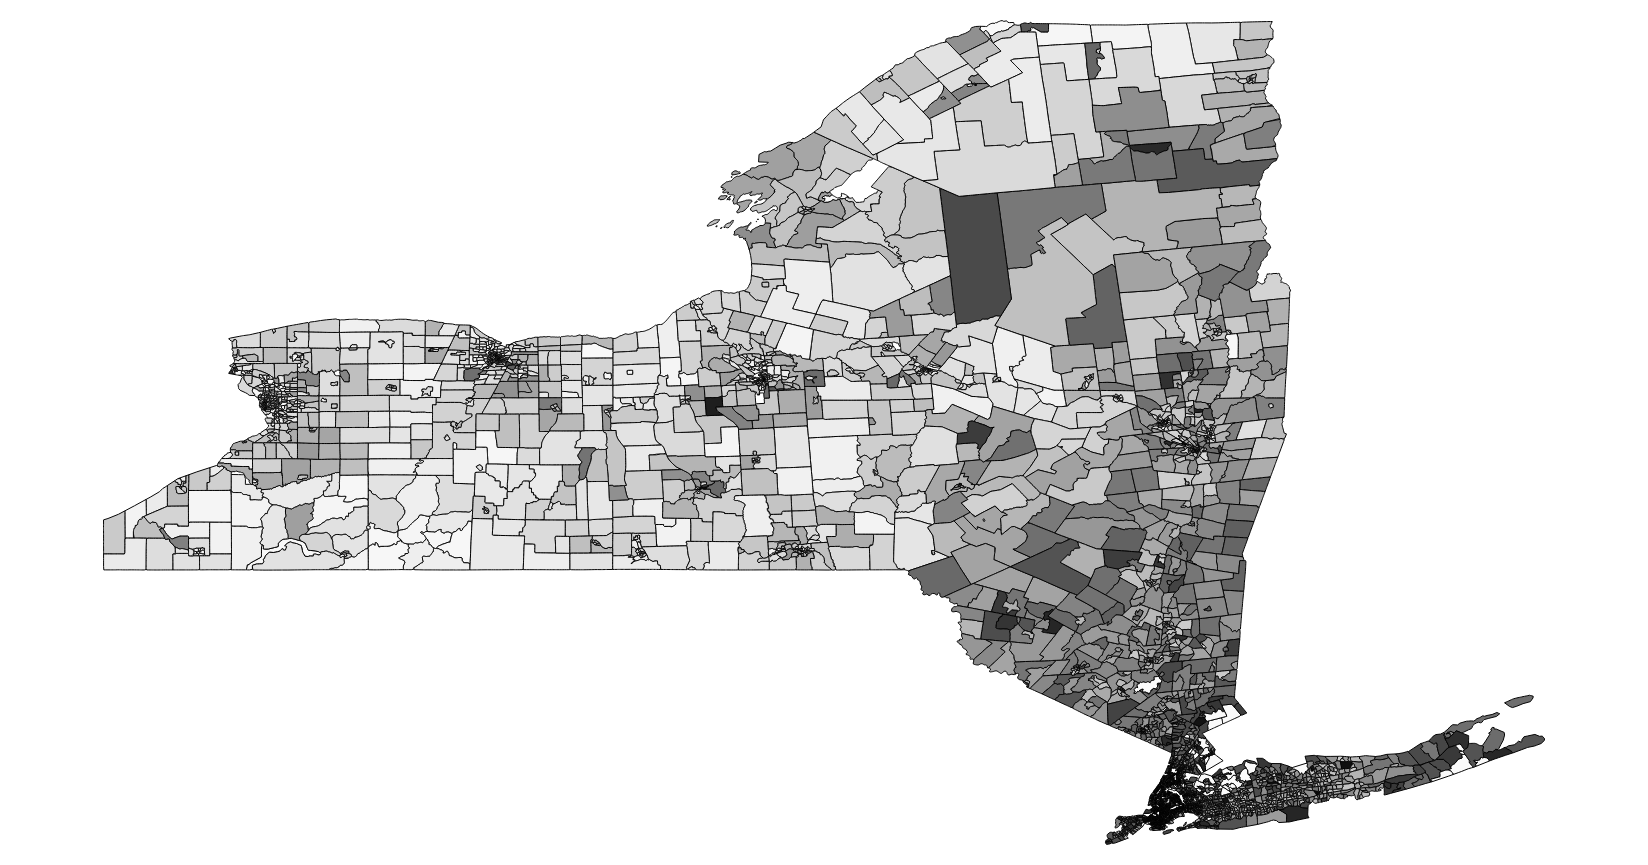
\includegraphics[scale=.4]{map_4}
\caption{This shows something}
\end{framed}
\end{figure}

So as not to have a ridiculous number of edges between the stores and the intermediaries, I've actually aggregated the number of edges by Census district. The reason for using this method to aggregate stores is because I am multiplying square footage of the stores by the property to more appropriately weight the value of the square footage (i.e. a store in new york city might be the same size as a store upstate, but it you might expect it to sell significantly more produce even though they are the same size. This is because the population density is much tighter in new york and the consumers might have more income to spend on produce in New York). I'm essentially assuming that when the stores choose how big they are, they value the properties based on how much they can how much one city versus anther translates into sales and they choose an optimal size appropriately. This is by no means meant to be an exact estimate and specifying a problem where store owners choose optimal square footage to meet demand would be a lot more complicated, it's only supposed to be better than a naive estimate of area by its self.

\begin{table}
\centering
\begin{framed}
\begin{tabular}{c|c|c|c|c}%
	Band&Average&Minimum&Maximum&Variance
    \csvreader[head to column names]{stores.csv}{}% use head of csv as column names
    {\\\hline \csvcoli & \csvcolii & \csvcoliii & \csvcoliv & \csvcolv}
\end{tabular}
\caption{Another table caption}
\end{framed}
\end{table}


\subsection{Edge Costs}

Basically, I set up a local instance of Open source routing machine and used OSRM.
The prices are measured in seconds.
The software loaded in a map and then it acts as a server that does routing.
I let it run on my computer, connect over the local network and it responds.

In applied mathematics, the method of contraction hierarchies is a technique to speed up shortest-path routing by first creating precomputed "contracted" versions of the connection graph. It can be regarded as a special case of "highway-node routing".

Contraction hierarchies can be used to generate shortest-path routes much more efficiently than Dijkstra's algorithm or previous highway-node routing approaches,[1] and is used in many advanced routing techniques. It is publicly available in open source software to calculate routes from one place to another.

The speeds are based on expected times on each road.

\begin{table}
\centering
\begin{framed}
\begin{tabular}{c|c|c|c|c}%
	Band&Average&Minimum&Maximum&Variance
    \csvreader[head to column names]{fp_edges.csv}{}% use head of csv as column names
    {\\\hline \csvcoli & \csvcolii & \csvcoliii & \csvcoliv & \csvcolv}
\end{tabular}
\caption{Another table caption}
\end{framed}
\end{table}

\begin{table}
\centering
\begin{framed}
\begin{tabular}{c|c|c|c|c}%
	Band&Average&Minimum&Maximum&Variance
    \csvreader[head to column names]{ps_edges.csv}{}% use head of csv as column names
    {\\\hline \csvcoli & \csvcolii & \csvcoliii & \csvcoliv & \csvcolv}
\end{tabular}
\caption{Another table caption}
\end{framed}
\end{table}





\chapter{Results}

\section{Onion Farms}

\begin{table}
\centering
\begin{framed}
\begin{tabular}{c|c|c|c}%
	Type&Average&Variance&Deviation
    \csvreader[head to column names]{price_49.csv}{}% use head of csv as column names
    {\\\hline \csvcoli & \csvcolii & \csvcoliii & \csvcoliv}
\end{tabular}
\caption{Another table caption}
\end{framed}
\end{table}

\begin{table}
\centering
\begin{framed}
\begin{tabular}{c|c|c|c|c}%
	Type&Max Price&Max County&Min Price&Min County
    \csvreader[head to column names]{county_49.csv}{}% use head of csv as column names
    {\\\hline \csvcoli & \csvcolii & \csvcoliii & \csvcoliv & \csvcolv}
\end{tabular}
\caption{Another table caption}
\end{framed}
\end{table}

\begin{figure}
\centering
\begin{framed}
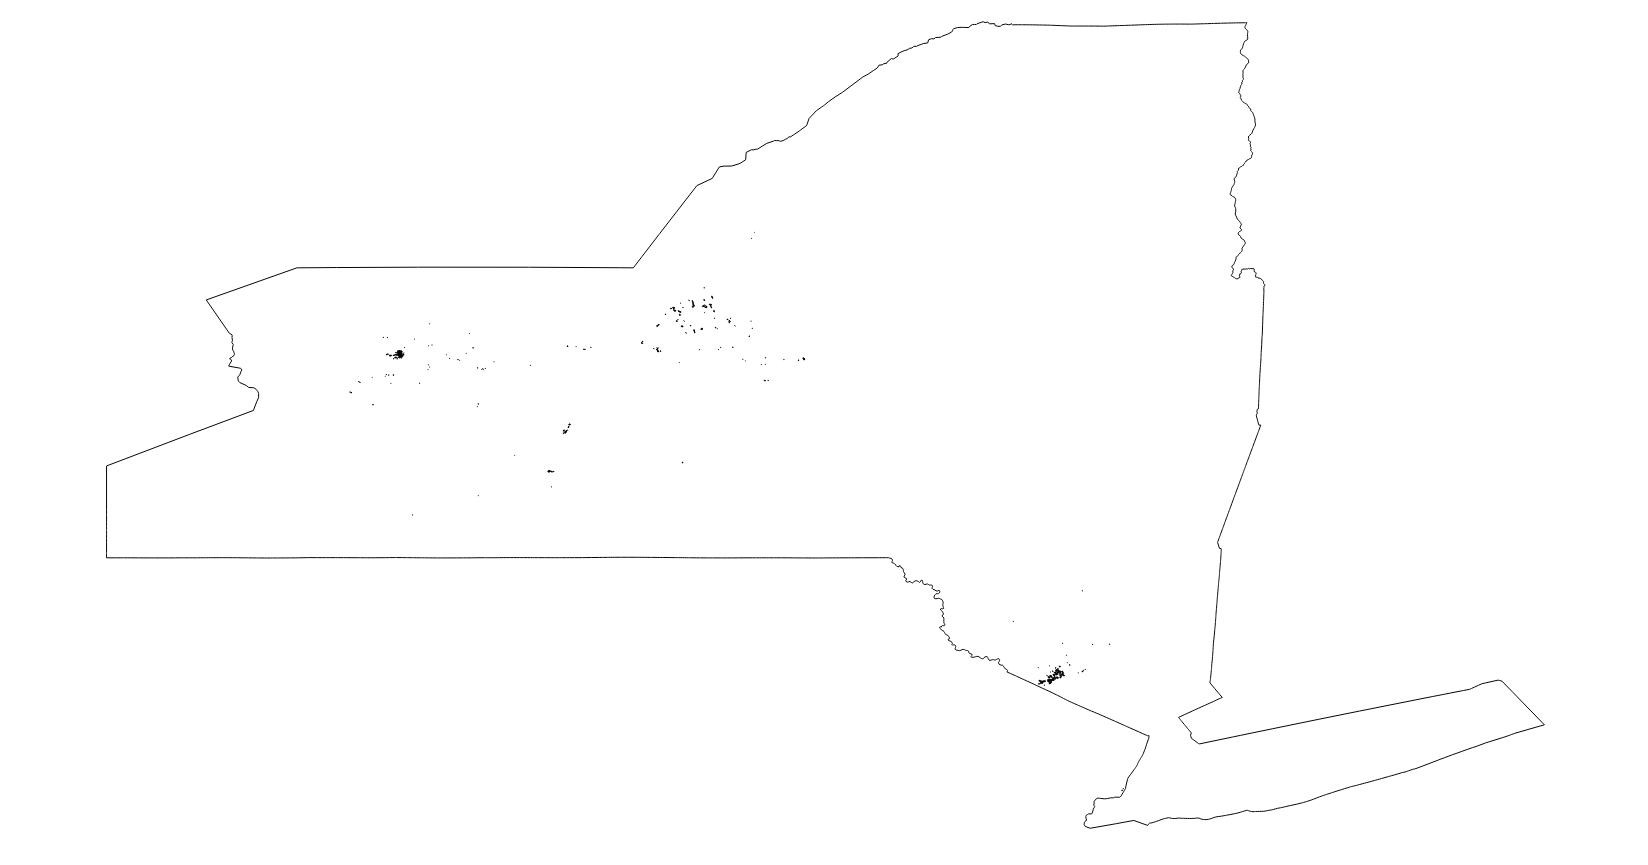
\includegraphics[scale=.4]{farms_49}
\caption{This shows something}
\end{framed}
\end{figure}

\begin{figure}
\centering
\begin{framed}
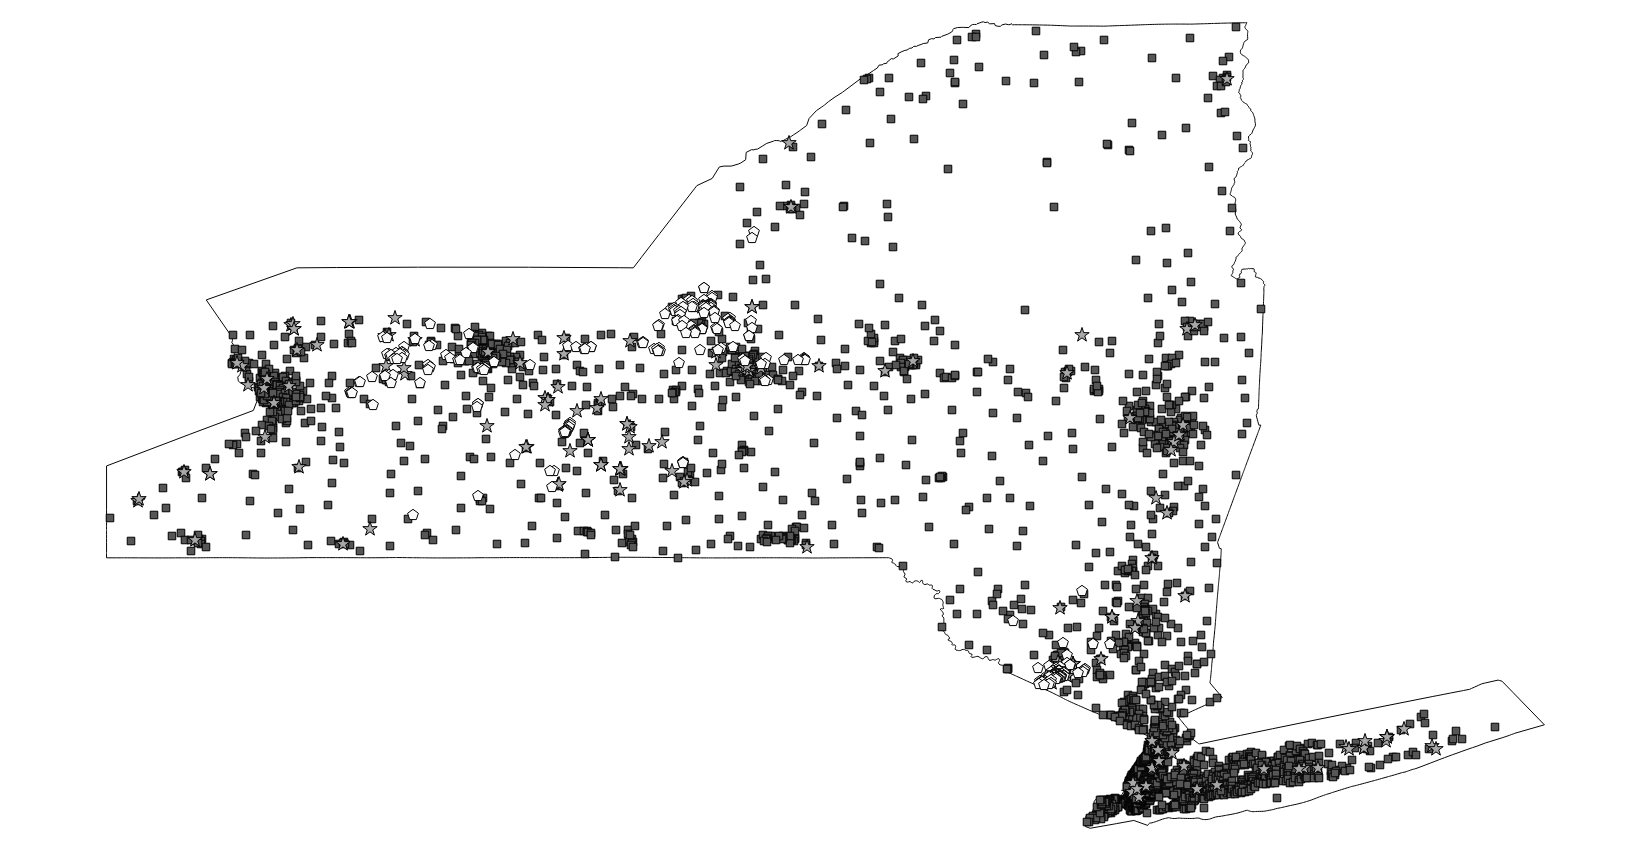
\includegraphics[scale=.4]{network_49}
\caption{This shows something}
\end{framed}
\end{figure}

\begin{figure}
\centering
\begin{framed}
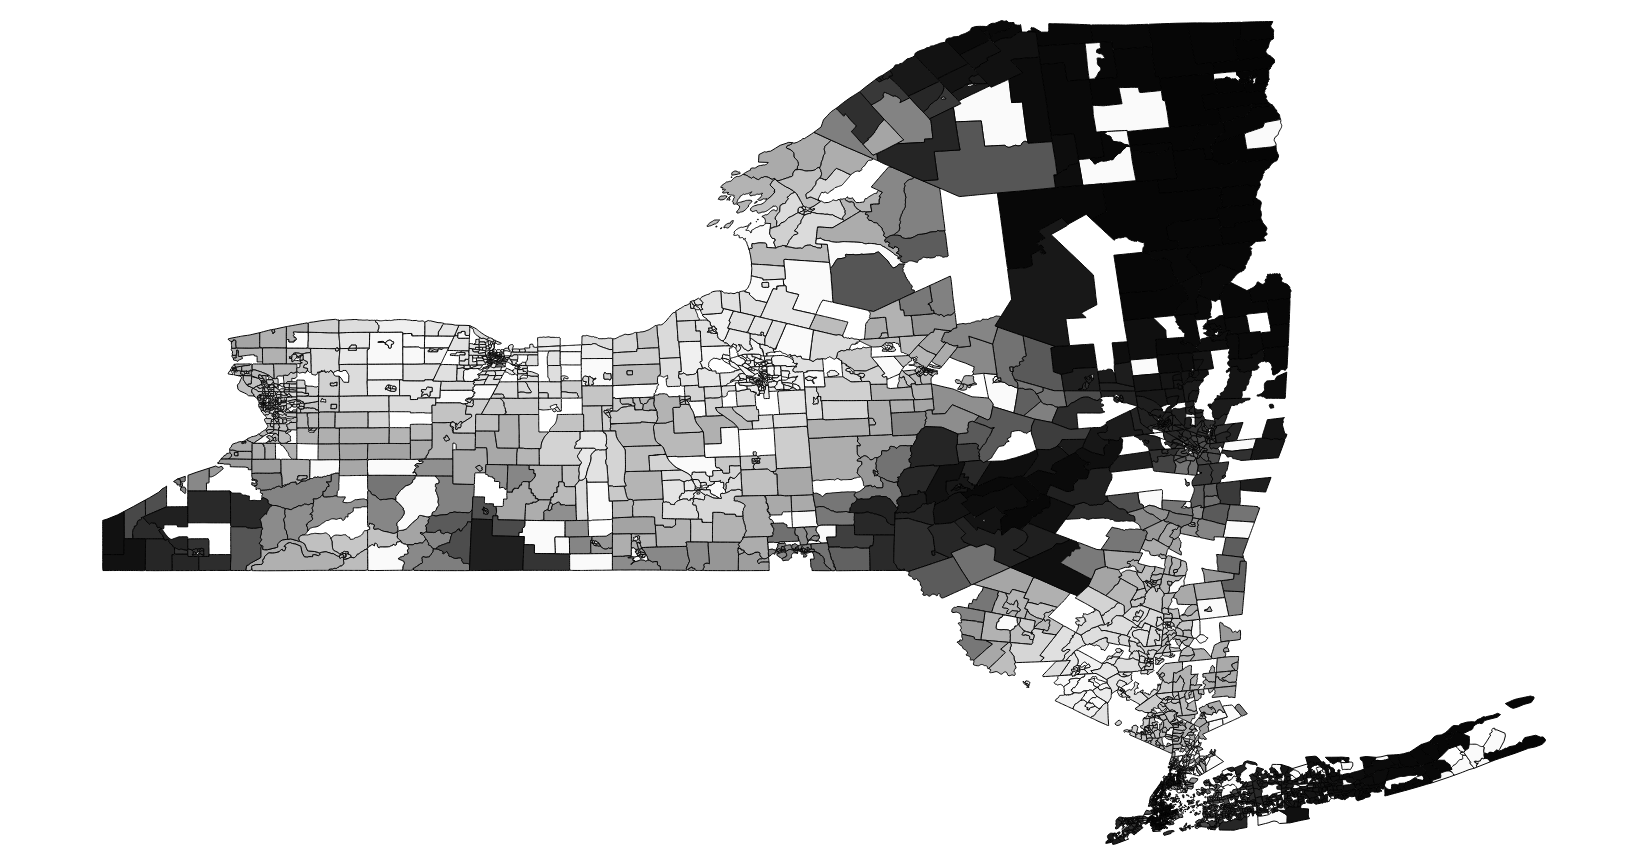
\includegraphics[scale=.4]{prices_49}
\caption{This shows something}
\end{framed}
\end{figure}

\section{Cherry Farms}

\begin{table}
\centering
\begin{framed}
\begin{tabular}{c|c|c|c}%
	Type&Average&Variance&Deviation
    \csvreader[head to column names]{price_66.csv}{}% use head of csv as column names
    {\\\hline \csvcoli & \csvcolii & \csvcoliii & \csvcoliv}
\end{tabular}
\caption{Another table caption}
\end{framed}
\end{table}

\begin{table}
\centering
\begin{framed}
\begin{tabular}{c|c|c|c|c}%
	Type&Max Price&Max County&Min Price&Min County
    \csvreader[head to column names]{county_66.csv}{}% use head of csv as column names
    {\\\hline \csvcoli & \csvcolii & \csvcoliii & \csvcoliv & \csvcolv}
\end{tabular}
\caption{Another table caption}
\end{framed}
\end{table}

\begin{figure}
\centering
\begin{framed}
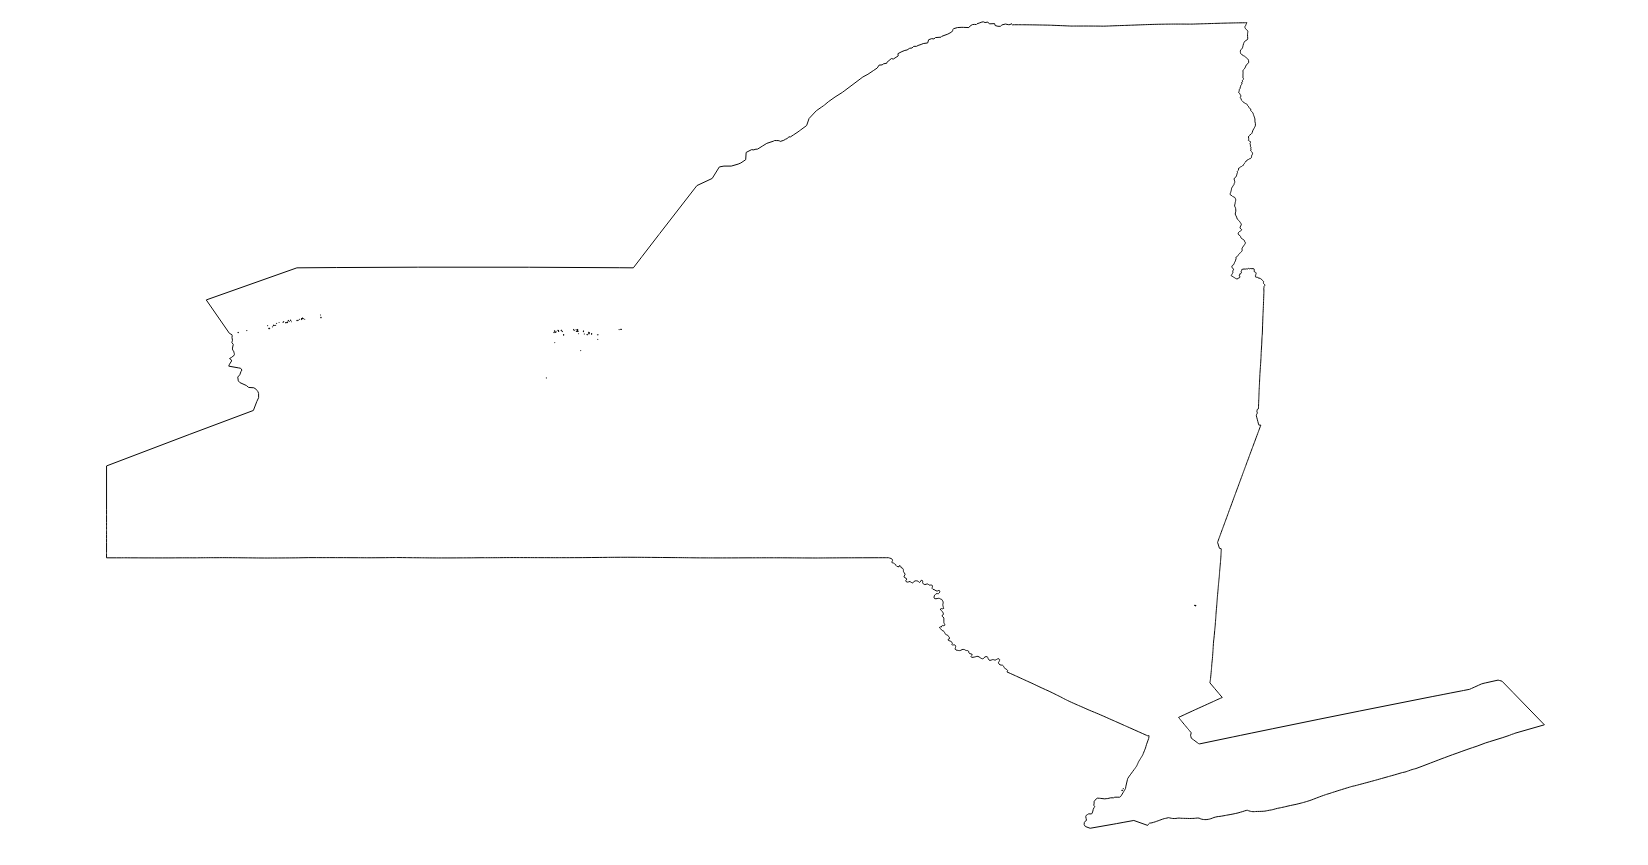
\includegraphics[scale=.4]{farms_66}
\caption{This shows something}
\end{framed}
\end{figure}

\begin{figure}
\centering
\begin{framed}
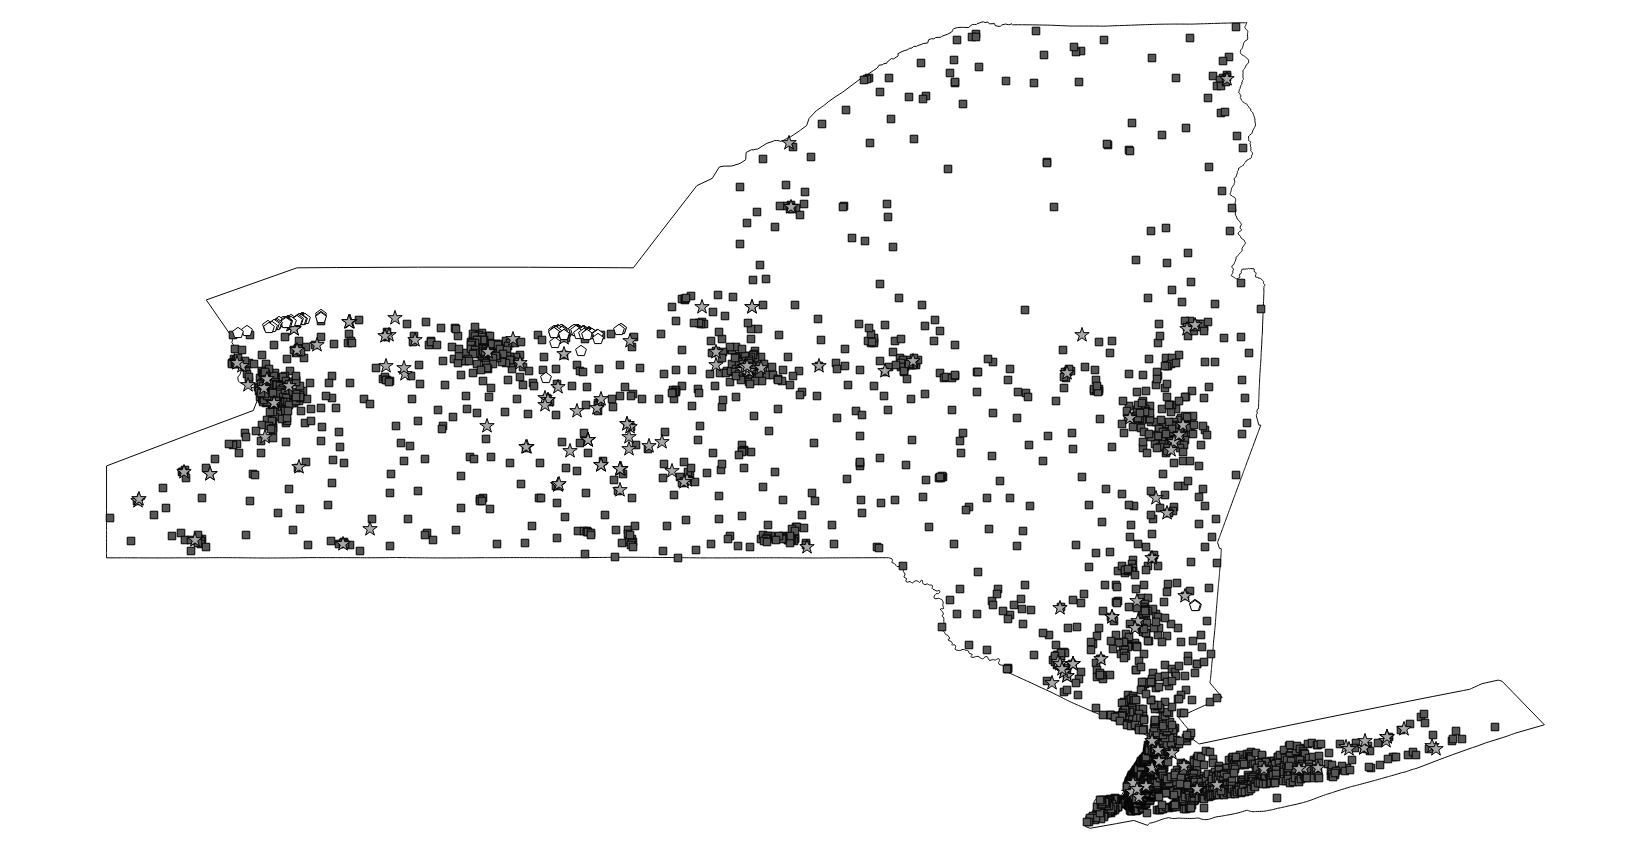
\includegraphics[scale=.4]{network_66}
\caption{This shows something}
\end{framed}
\end{figure}

\begin{figure}
\centering
\begin{framed}
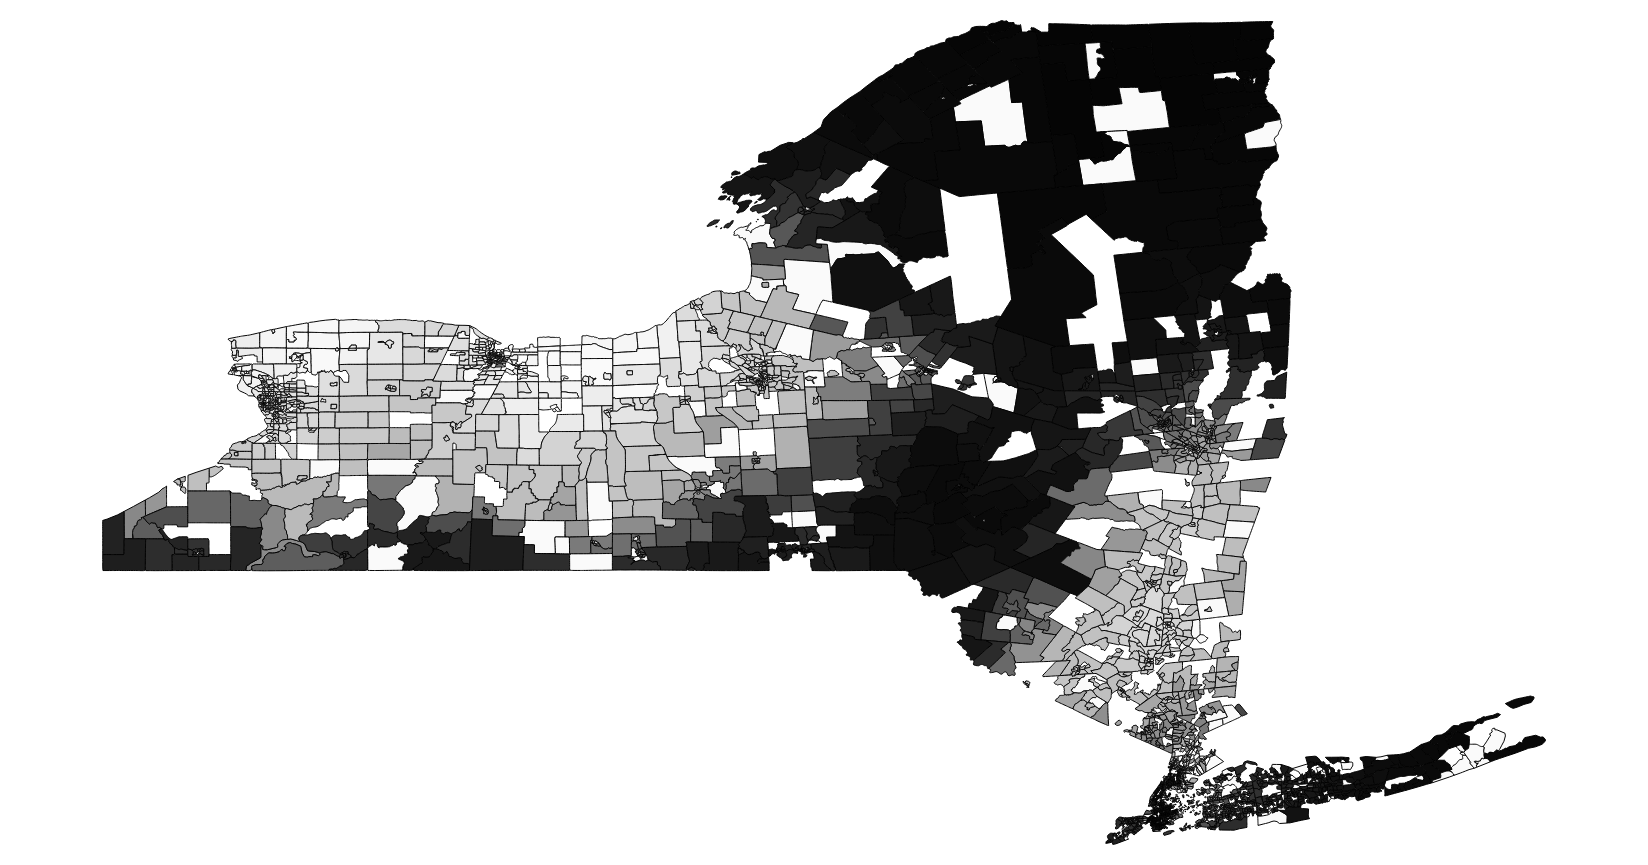
\includegraphics[scale=.4]{prices_66}
\caption{This shows something}
\end{framed}
\end{figure}

\section{Grape Farms}

\begin{table}
\centering
\begin{framed}
\begin{tabular}{c|c|c|c}%
	Type&Average&Variance&Deviation
    \csvreader[head to column names]{price_69.csv}{}% use head of csv as column names
    {\\\hline \csvcoli & \csvcolii & \csvcoliii & \csvcoliv}
\end{tabular}
\caption{Another table caption}
\end{framed}
\end{table}

\begin{table}
\centering
\begin{framed}
\begin{tabular}{c|c|c|c|c}%
	Type&Max Price&Max County&Min Price&Min County
    \csvreader[head to column names]{county_69.csv}{}% use head of csv as column names
    {\\\hline \csvcoli & \csvcolii & \csvcoliii & \csvcoliv & \csvcolv}
\end{tabular}
\caption{Another table caption}
\end{framed}
\end{table}

\begin{figure}
\centering
\begin{framed}
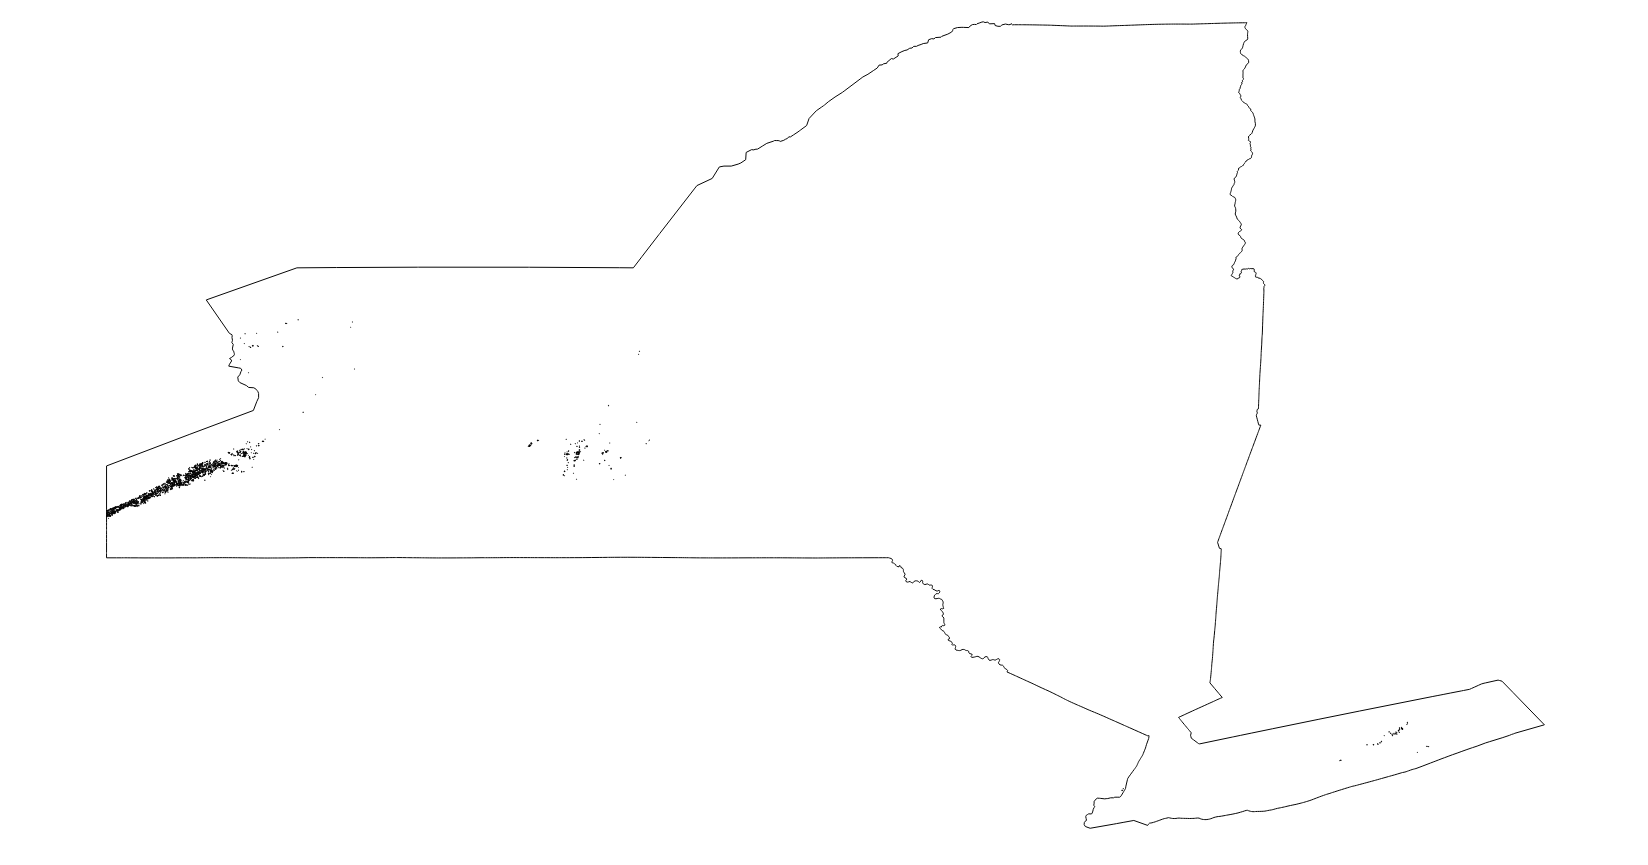
\includegraphics[scale=.4]{farms_69}
\caption{This shows something}
\end{framed}
\end{figure}

\begin{figure}
\centering
\begin{framed}
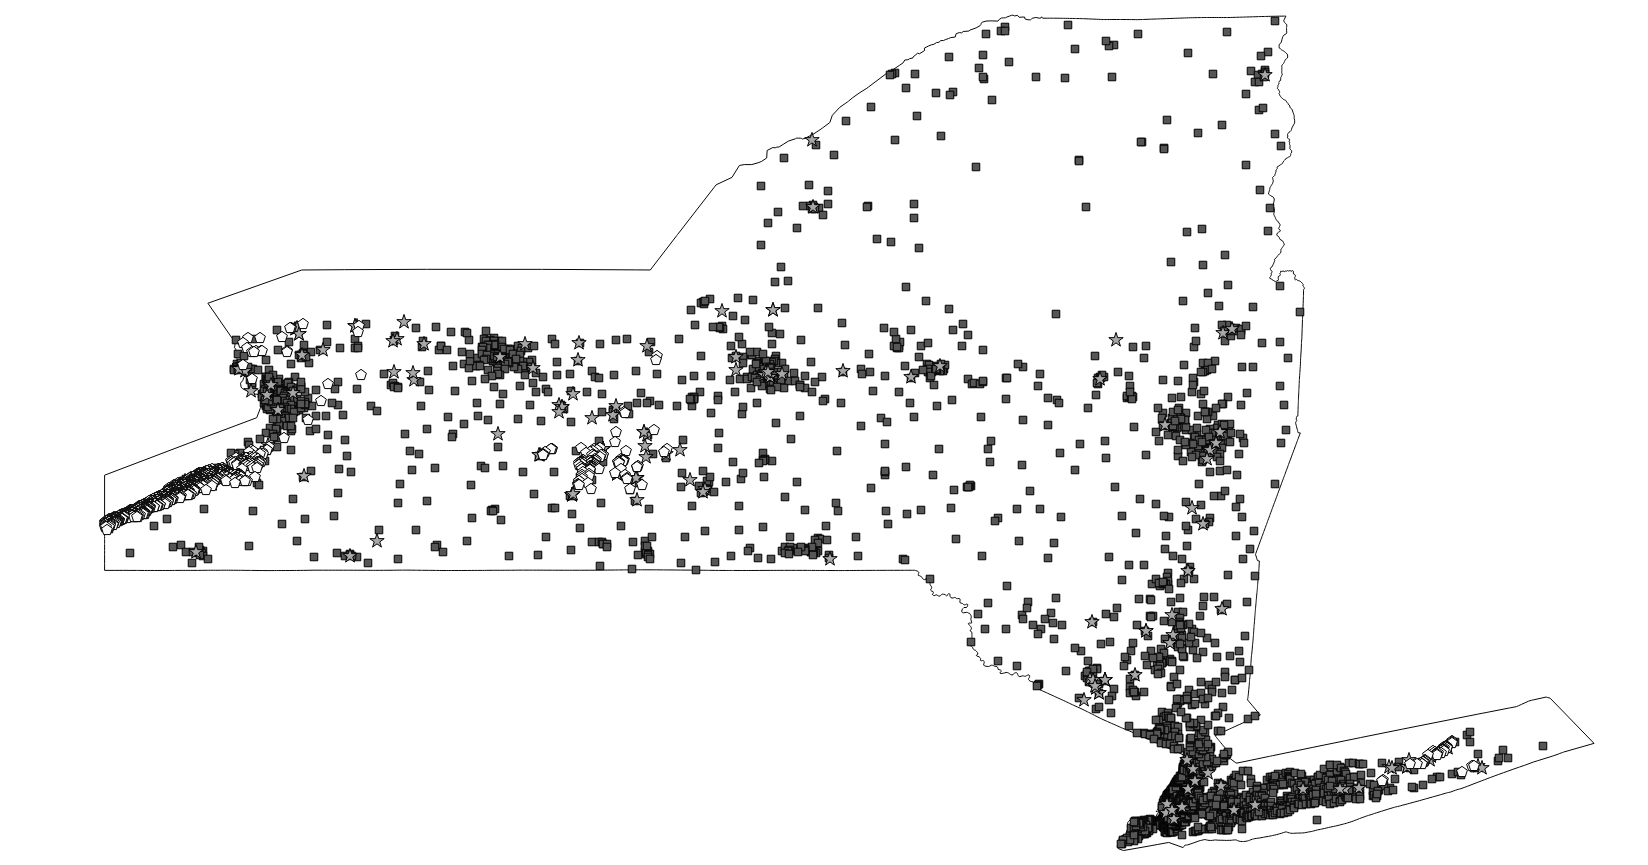
\includegraphics[scale=.4]{network_69}
\caption{This shows something}
\end{framed}
\end{figure}

\begin{figure}
\centering
\begin{framed}
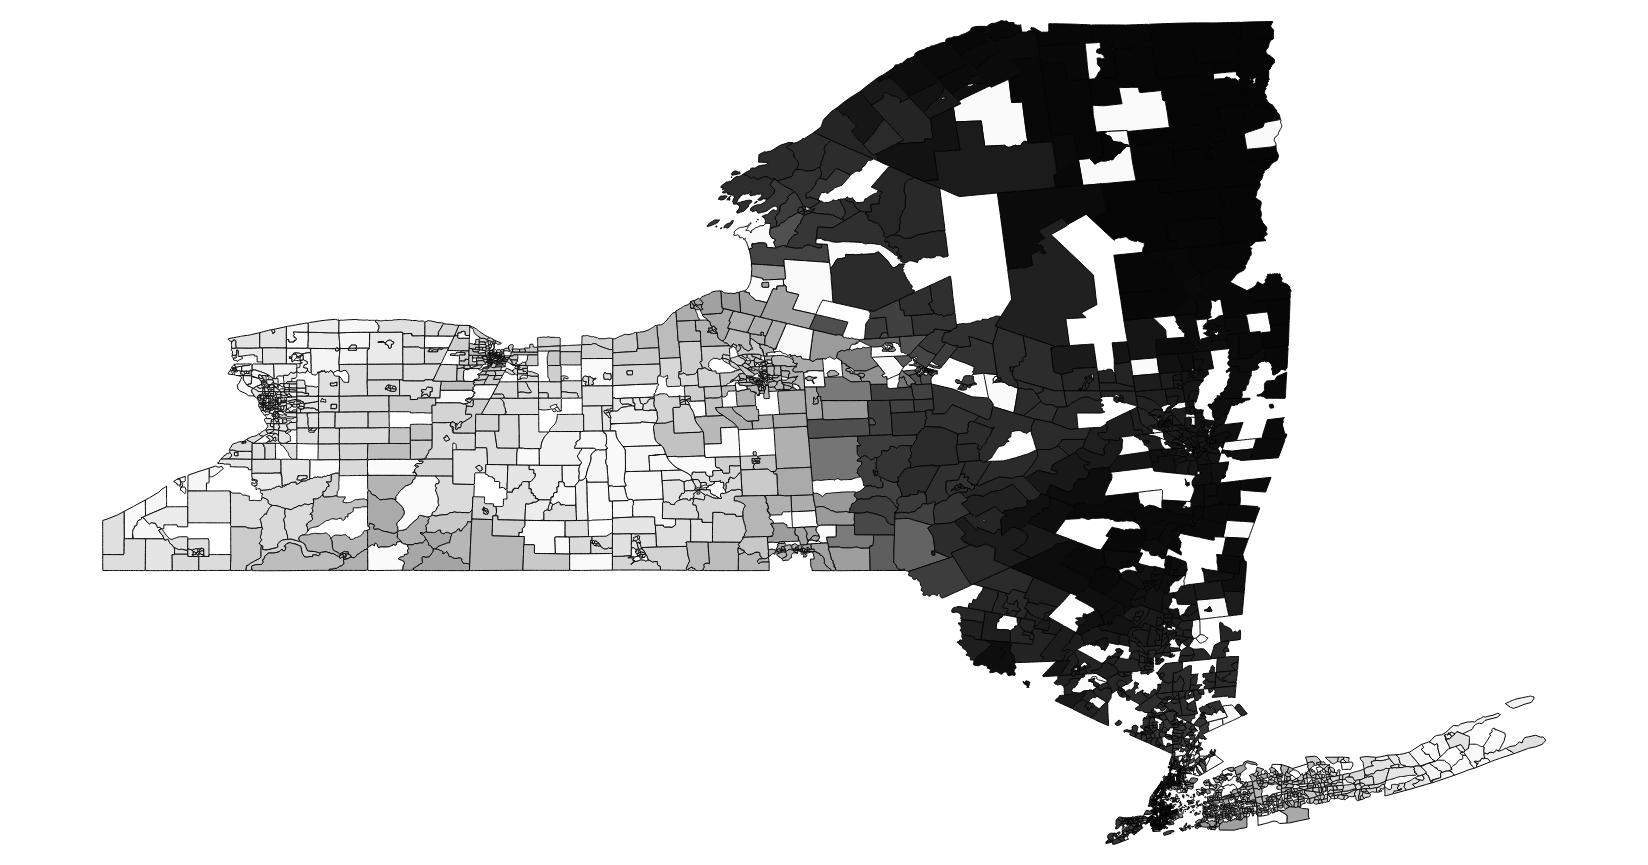
\includegraphics[scale=.4]{prices_69}
\caption{This shows something}
\end{framed}
\end{figure}

\section{Cabbage Farms}

\begin{table}
\centering
\begin{framed}
\begin{tabular}{c|c|c|c}%
	Type&Average&Variance&Deviation
    \csvreader[head to column names]{price_243.csv}{}% use head of csv as column names
    {\\\hline \csvcoli & \csvcolii & \csvcoliii & \csvcoliv}
\end{tabular}
\caption{Another table caption}
\end{framed}
\end{table}

\begin{table}
\centering
\begin{framed}
\begin{tabular}{c|c|c|c|c}%
	Type&Max Price&Max County&Min Price&Min County
    \csvreader[head to column names]{county_243.csv}{}% use head of csv as column names
    {\\\hline \csvcoli & \csvcolii & \csvcoliii & \csvcoliv & \csvcolv}
\end{tabular}
\caption{Another table caption}
\end{framed}
\end{table}

\begin{figure}
\centering
\begin{framed}
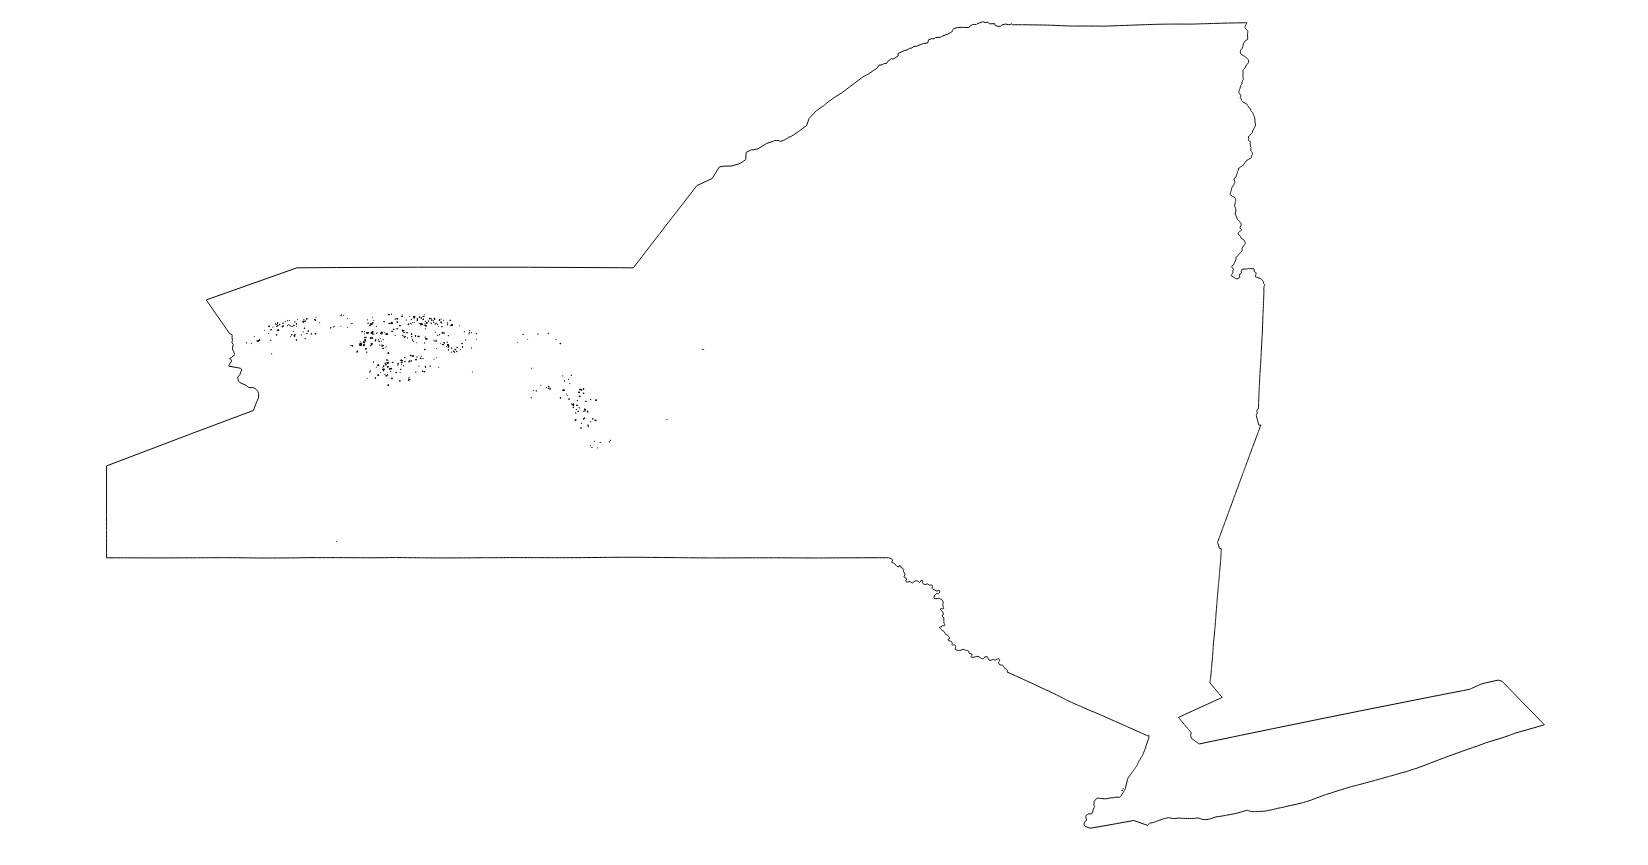
\includegraphics[scale=.4]{farms_243}
\caption{This shows something}
\end{framed}
\end{figure}

\begin{figure}
\centering
\begin{framed}
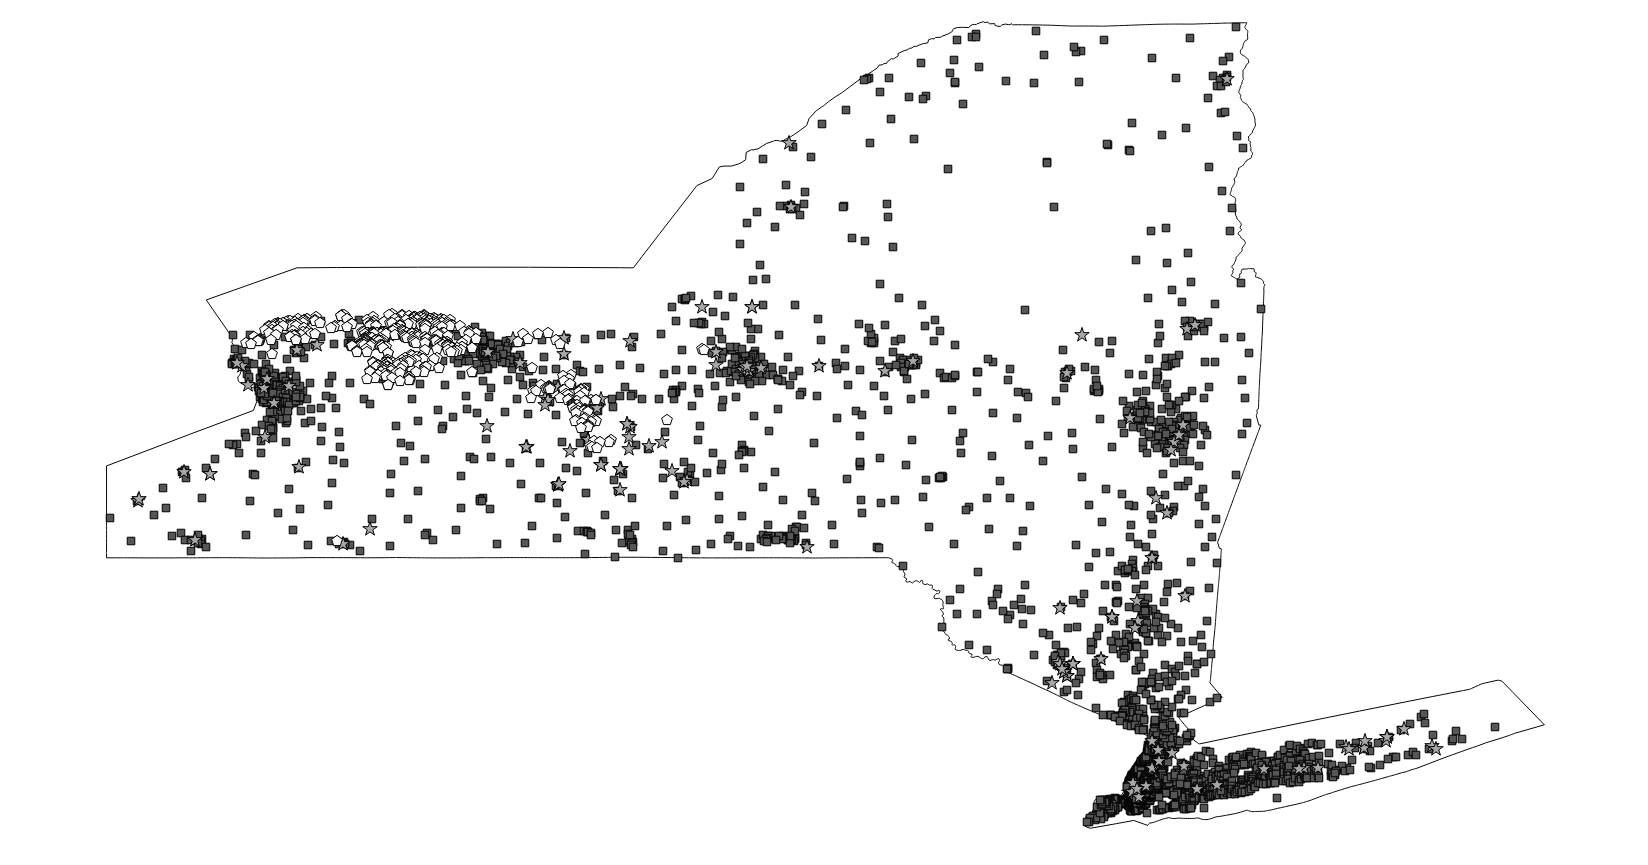
\includegraphics[scale=.4]{network_243}
\caption{This shows something}
\end{framed}
\end{figure}

\begin{figure}
\centering
\begin{framed}
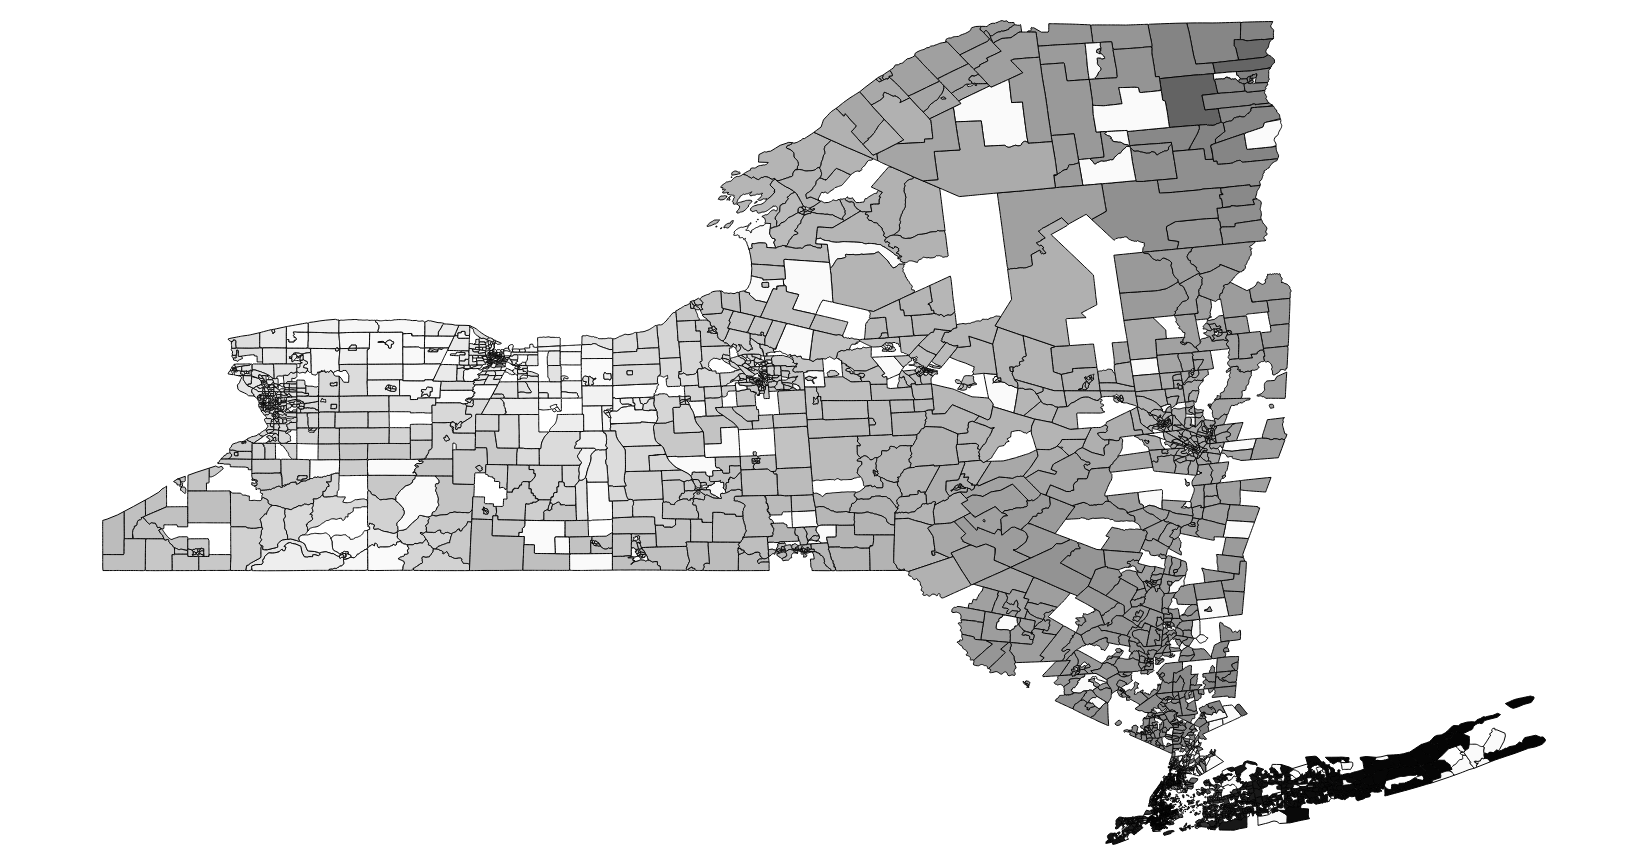
\includegraphics[scale=.4]{prices_243}
\caption{This shows something}
\end{framed}
\end{figure}


\chapter{Discussion}




\section{Robustness of Solutions}
I tried to perturb the solution to the linear program.
Greater than the maximum
Less than the maximum
less than the minimum
greater than the minimum

Although it changed the results it didn't really change things drastically.
To be honest, I think the changes have more to do with rounding errors related to the way that python stores floating point numbers rather than actual differences to the solution. When the value of the objective function is parsed from the solution file into a python float the last decimal point may not be accurate. 
As you can expect the numbers didn't differ drastically.

I've included a table of the differences between table XX and table YY as a quick reference so you can get a sense of what I found. I can provide the other difference tables as .csv files upon request if you want to look through them in detail. They can also be generated using the git repository.

\section{Comparing Different Results}


So, all the results ended up looking pretty similar. I guess that happens because of the fact that processors and stores stay pretty the much the same for each of the goods.

So, cabbages actually being interesting. The variance in the prices calculated by the algorithm is a lot lower. Considering the that store and for the most part intermediate processors stay constant between the various bands in the problem, it becomes obvious the aspect of the network that changed is the farms. 

As you can see there are more cabbage farms. They are more spread apart and there is less variance in terms of their size.

\subsection{Farms}

\begin{table}
\centering
\begin{framed}
\begin{tabular}{c|c|c|c|c|c}%
	Band&Total&Average&Minimum&Maximum&Variance
    \csvreader[head to column names]{farms.csv}{}% use head of csv as column names
    {\\\hline \csvcoli & \csvcolii & \csvcoliii & \csvcoliv& \csvcolv & \csvcolvi}
\end{tabular}
\caption{Another table caption}
\end{framed}
\end{table}

\begin{table}
\centering
\begin{framed}
\begin{tabular}{c|c|c|c}%
	Band&Average&Variance&Deviation
    \csvreader[head to column names]{farm_price.csv}{}% use head of csv as column names
    {\\\hline \csvcoli & \csvcolii & \csvcoliii & \csvcoliv}
\end{tabular}
\caption{Another table caption}
\end{framed}
\end{table}

\begin{table}
\centering
\begin{framed}
\begin{tabular}{c|c|c|c|c}%
	Band&Max Price&Max County&Min Price&Min County
    \csvreader[head to column names]{farm_county.csv}{}% use head of csv as column names
    {\\\hline \csvcoli & \csvcolii & \csvcoliii & \csvcoliv & \csvcolv}
\end{tabular}
\caption{Another table caption}
\end{framed}
\end{table}

\subsection{Intermediate Processors}

\begin{table}
\centering
\begin{framed}
\begin{tabular}{c|c}%
	Band & Count
    \csvreader[head to column names]{procs.csv}{}% use head of csv as column names
    {\\\hline \csvcoli & \csvcolii}
\end{tabular}
\caption{Another table caption}
\end{framed}
\end{table}


\begin{table}
\centering
\begin{framed}
\begin{tabular}{c|c|c|c}%
	Band&Average&Variance&Deviation
    \csvreader[head to column names]{proc_price.csv}{}% use head of csv as column names
    {\\\hline \csvcoli & \csvcolii & \csvcoliii & \csvcoliv}
\end{tabular}
\caption{Another table caption}
\end{framed}
\end{table}

\begin{table}
\centering
\begin{framed}
\begin{tabular}{c|c|c|c|c}%
	Band&Max Price&Max County&Min Price&Min County
    \csvreader[head to column names]{proc_county.csv}{}% use head of csv as column names
    {\\\hline \csvcoli & \csvcolii & \csvcoliii & \csvcoliv & \csvcolv}
\end{tabular}
\caption{Another table caption}
\end{framed}
\end{table}


\begin{figure}
\centering
\begin{framed}
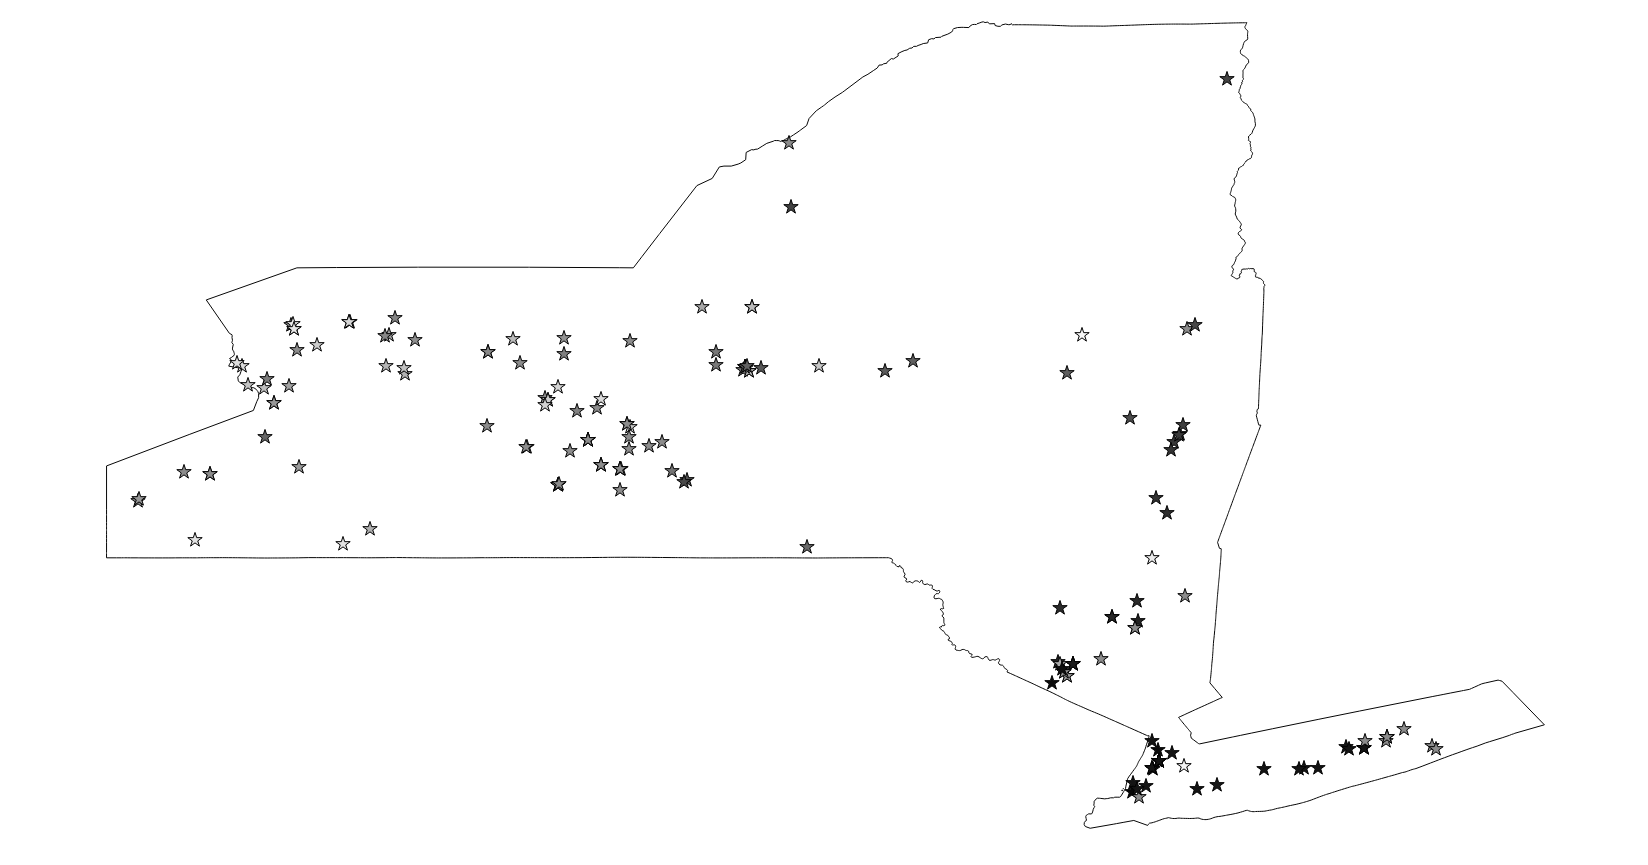
\includegraphics[scale=.4]{procs_243_49}
\caption{This shows something}
\end{framed}
\end{figure}

\begin{figure}
\centering
\begin{framed}
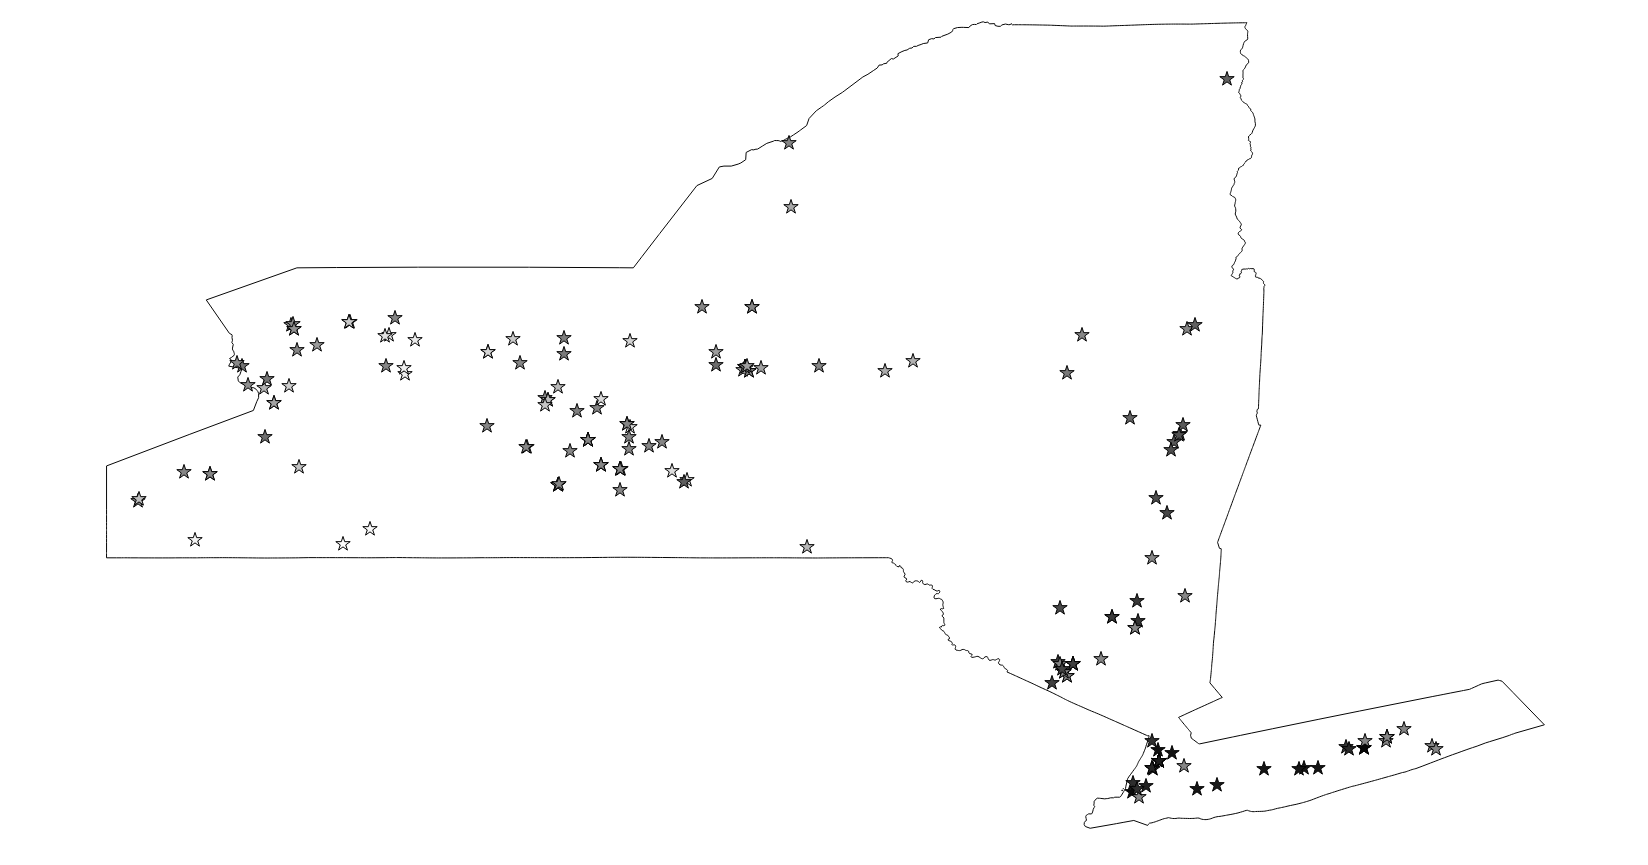
\includegraphics[scale=.4]{procs_243_66}
\caption{This shows something}
\end{framed}
\end{figure}

\begin{figure}
\centering
\begin{framed}
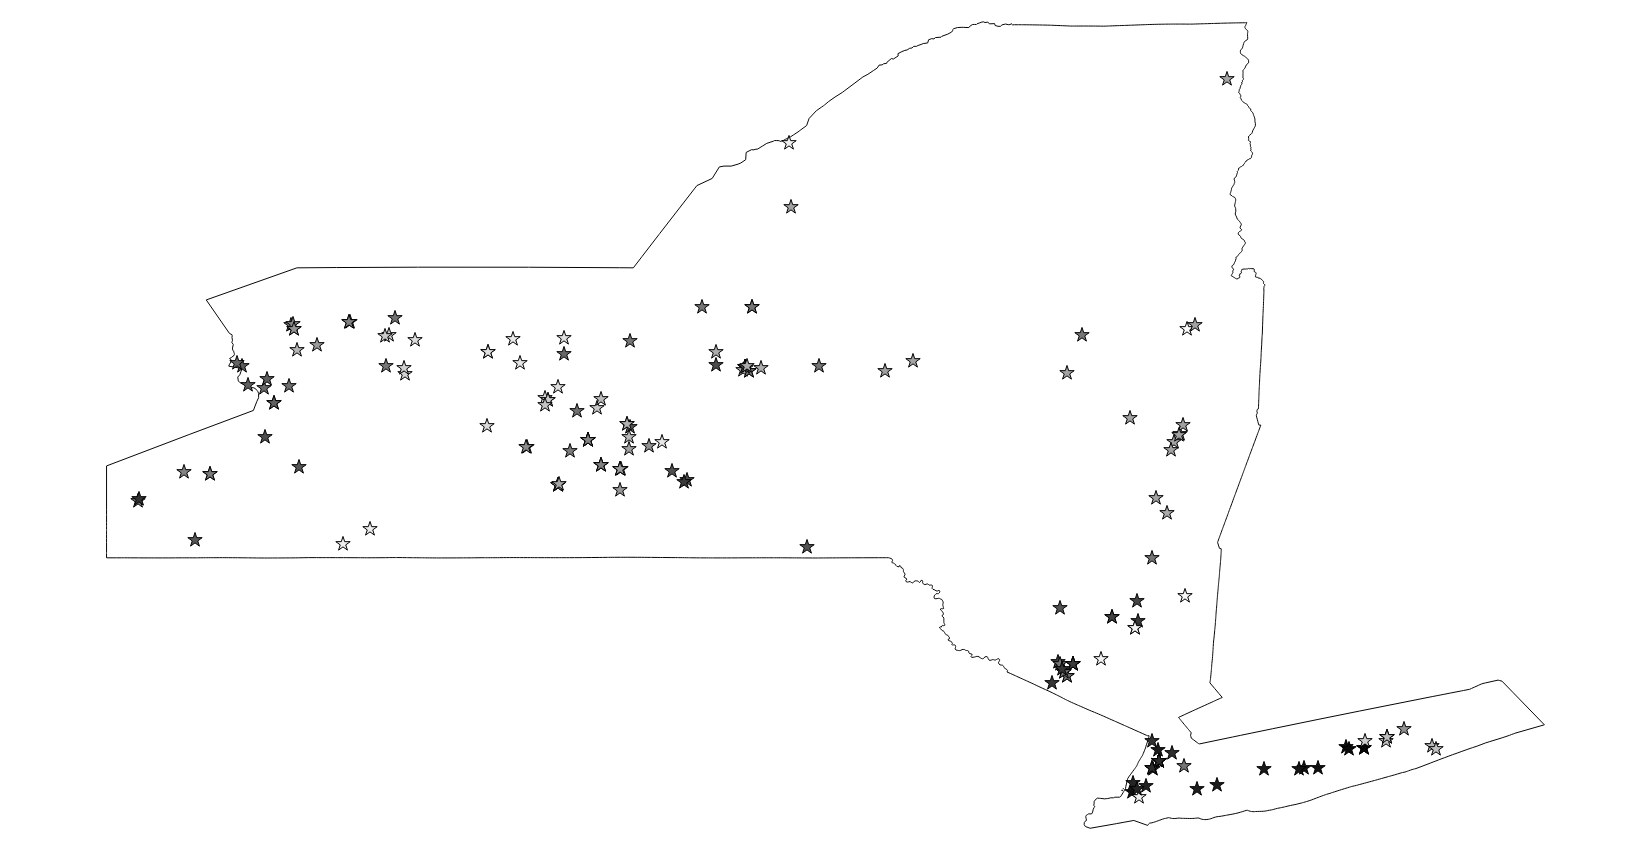
\includegraphics[scale=.4]{procs_243_69}
\caption{This shows something}
\end{framed}
\end{figure}

\subsection{Stores}

\begin{figure}
\centering
\begin{framed}
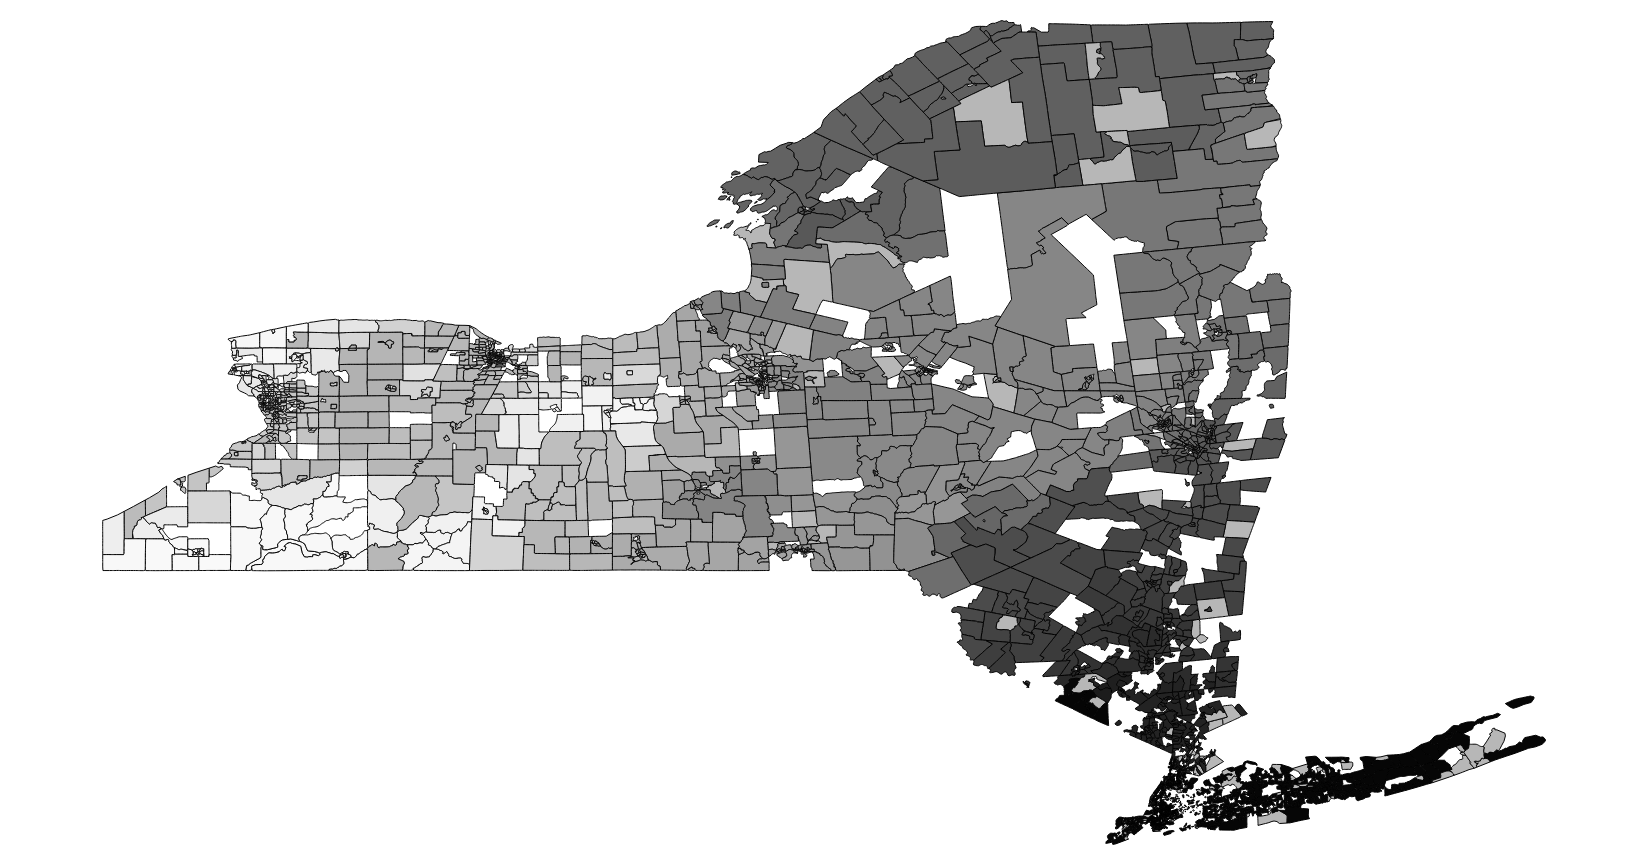
\includegraphics[scale=.4]{stores_243_49}
\caption{This shows something}
\end{framed}
\end{figure}

\begin{figure}
\centering
\begin{framed}
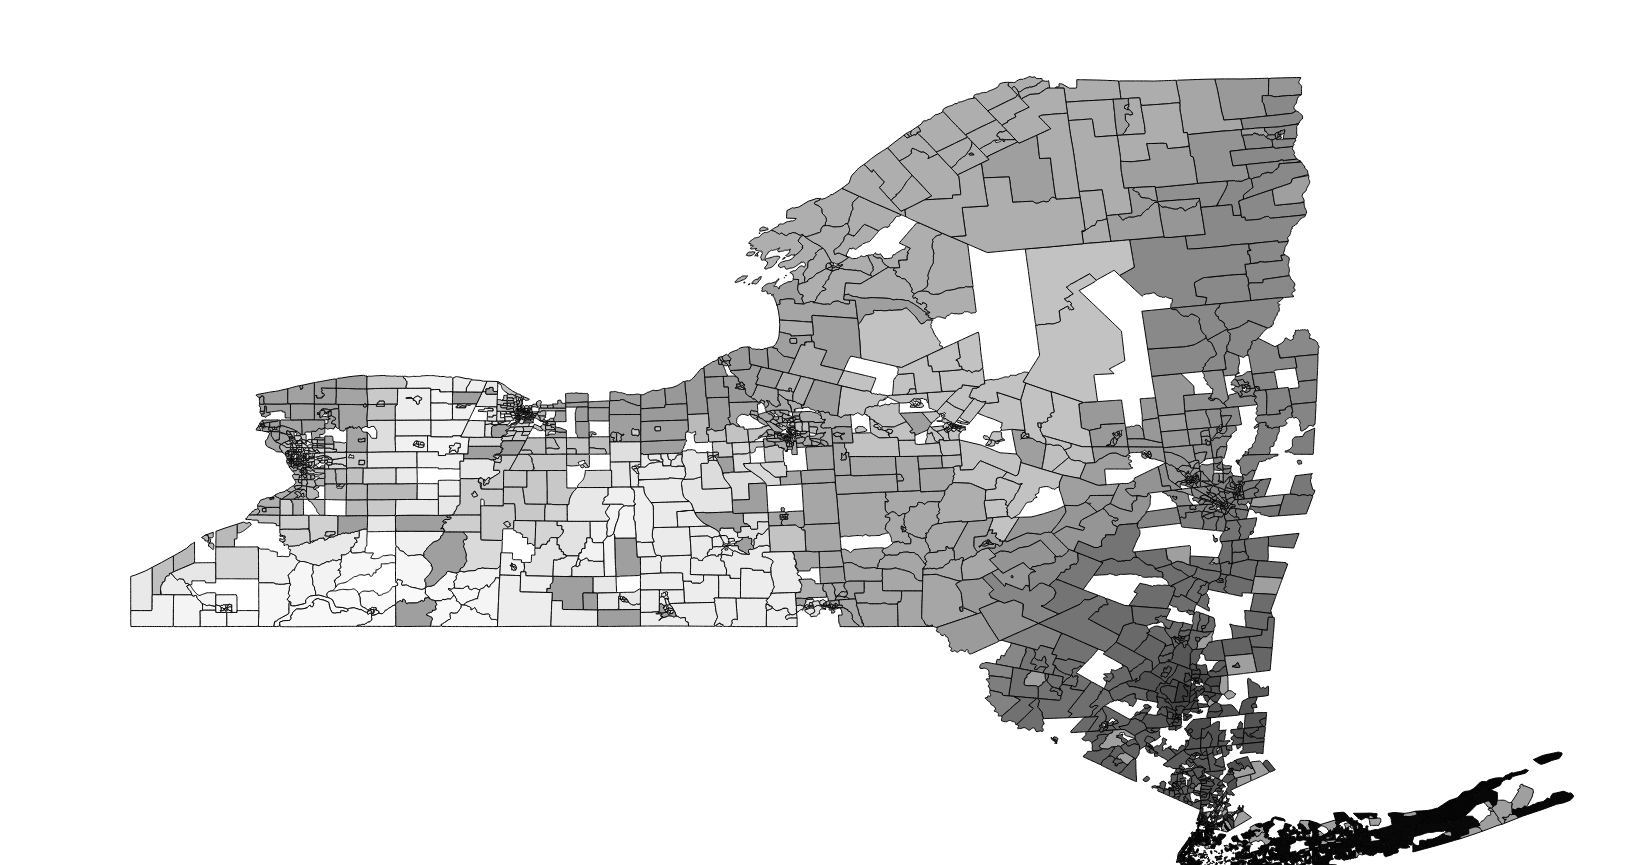
\includegraphics[scale=.4]{stores_243_66}
\caption{This shows something}
\end{framed}
\end{figure}

\begin{figure}
\centering
\begin{framed}
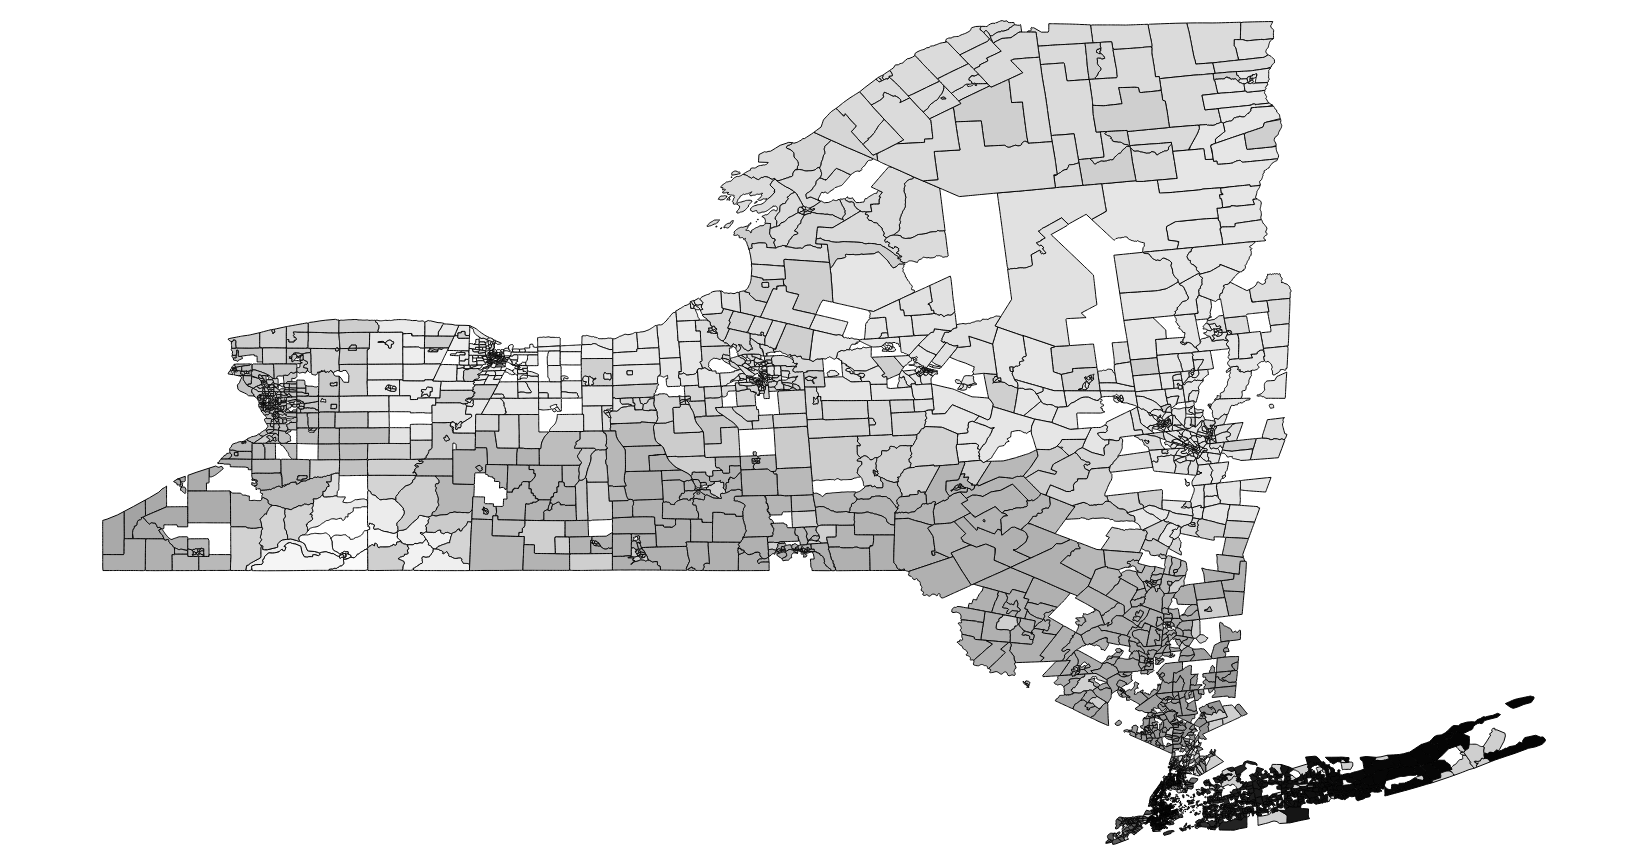
\includegraphics[scale=.4]{stores_243_69}
\caption{This shows something}
\end{framed}
\end{figure}

\begin{table}
\centering
\begin{framed}
\begin{tabular}{c|c|c|c}%
	Band&Average&Variance&Deviation
    \csvreader[head to column names]{store_price.csv}{}% use head of csv as column names
    {\\\hline \csvcoli & \csvcolii & \csvcoliii & \csvcoliv}
\end{tabular}
\caption{Another table caption}
\end{framed}
\end{table}


\begin{table}
\centering
\begin{framed}
\begin{tabular}{c|c|c|c|c}%
	Band&Max Price&Max County&Min Price&Min County
    \csvreader[head to column names]{store_county.csv}{}% use head of csv as column names
    {\\\hline \csvcoli & \csvcolii & \csvcoliii & \csvcoliv & \csvcolv}
\end{tabular}
\caption{Another table caption}
\end{framed}
\end{table}




\section{Checking the Uniqueness of Results}

I think this more has to do with a rounding error, rather than an issue with the data.
One key question is how I've skipped doing exclusion restrictions and the such to do my model.

The other question is how I've come up with point estimates when most empirical models come up with ranges.

The final thing is it might be foolish to look at the data in this way. I've probably lost a lot by ignoring the traditional techniques economist use make estimates about supply and demand. That being said, I think there is something here. There is a ton of potential in refining this technique more and more so that it's as polished as the techniques involved with ordinary least squares


\section{Transportation Problem Assumptions}

Despite the possibilities, prices in a transportation problem aren't a perfect analogue to market prices. Transportation problems assume firms coordinate to reduce total transportation costs. Additionally, prices in the problem only reflect linear transportation costs. To make the problem more realistic, we can increase all prices by a constant amount to reflect inputs (assuming constant returns to scale). Under this change, the solution is still optimal from a social planning perspective. 

Additionally, I am looking into better specifying the transportation problem using the Google Maps and MapQuest API.  My specification makes assumptions about connections between farms, factories, and retailers that may not exist for contractual reasons. In reality, fresh produce can be altered or stored at intermediaries, there may be capacities on the intermediate nodes, and intermediate nodes that buy less than 10,000 dollars of produce. 

Finally, I under-estimate costs because New York exports fresh produce. Adding demand from out-of-state increases costs in-state.  That being said, the estimated prices are still economically significant without exports. They represent a minimum for prices; adding additional demand from out-of-state increases costs in-state. Additionally, most of the categories of produce have a short shelf life and are exported in insignificant quantities with the exception of apples.

\chapter{Conclusion}
Instead of just jumping into my project. I figured I wanted to take a moment to reflect and explain why I've done what I've done. I've brought together a lot of cool tools from mapping and geographic imaging, optimization, and of course economics. I've tried my best to fit these tools together in a way that makes sense, but that's one of the hard things about looking about using a well established tool in an unconventional way. In some ways, it may not make sense. Either way, I definitely want to say it's been a fun and exciting process to see the resources that are out there beyond FRED, the BLS, and NCYS and would highly recommend to others to check it out and not be afraid when the file extension isn't .csv.

The second thing is Food is super complicated, I've created a model where I tried to capture the elements of the food transportation system that I thought were important. Obviously, there is room for improvement

\pagebreak

\begin{thebibliography}{99}
\bibitem{Bernell}Bernell, S., Weber, B., {\&} Edwards, M. (2006). Restricted Opportunities, Personal Choices, Ineffective Policies: What Explains Food Insecurity in Oregon? Journal of Agricultural and Resource Economics, 31(2), 193-211. 
\bibitem{Chung} Chung, Chanjin, and Samuel L. Myers. "Do the Poor Pay More for Food? An Analysis of Grocery Store Availability and Food Price Disparities." The Journal of Consumer Affairs 33.2 (1999): 276-96.
\bibitem{Cook} Cook, W. J., Cunningham, W. H., Pulleyblank, W. R.,  {\&}  Schrijver, A. (1998). Combinatorial optimization (pp. 91-126). New York: John Wiley  {\&}  Sons.
\bibitem{Hwang} Hwang, M., {\&} Smith, M. (2012). Integrating publicly available web mapping tools for cartographic visualization of community food insecurity: A prototype. GeoJournal, 77(1), 47-62.
\bibitem{Just} Just, R., {\&} Weninger, Q. (1997). Economic Evaluation of the Farmers' Market Nutrition Program. American Journal of Agricultural Economics, 79(3), 902-917.
\bibitem{Larson} Larson, J., {\&} Moseley, W. (2012). Reaching the limits: A geographic approach for understanding food insecurity and household hunger mitigation strategies in Minneapolis-Saint Paul, USA. GeoJournal, 77(1), 1-12.
\bibitem{Stewart} Stewart, T., {\&} Ittmann, H. (1979). Two-Stage Optimization in a Transportation Problem. The Journal of the Operational Research Society, 30(10), 897-904.

%Site econometric study multi-level


\end{thebibliography}



\end{document}